% Plantilla de memoria Universidad de los Andes
% para usuarios de pdfLaTeX.
%
% Jaime Cisternas, Santiago, junio de 2004, agosto 2010
%
% Necesita todos los archivos *.tex llamados en las
% sentencias \input{} (cap1, cap2,...)
% ademas de buc.bib y las figuras.
%
% El archivo setspace.sty permite especificar el espaciado
% entre las lineas. Los archivos newapa.sty y newapa.bst
% especifican el formato de la bibliografia.
%
% Para compilar :                    pdflatex memoria
% Para generar la bibliografia :     bibtex memoria, pdflatex memoria.tex (dos veces)

\documentclass[12pt]{report}

% El archivo siguiente contiene todos los detalles
% finos del formato de la memoria.
% No es necesario modificarlo.

% Definiciones basicas de LaTeX para la memoria
%
% No modificar las lineas a continuacion a menos
% de estar muy seguro de lo que se esta haciendo!!
%
% Jaime Cisternas, julio 2004, agosto 2010

% <jcisternas@uandes.cl> 

%%%%%%%%%%%%%%%%%%%%%%%%%%%%%%%%%%%%%%%%%%%%%%%%%%%%%%%%%%%%%%%%%%%%%

% Carga librerias utiles con simbolos y estructuras
\usepackage{amsfonts}
\usepackage{amssymb}
\usepackage{amsmath}   
\usepackage{amsthm}
\usepackage{latexsym}
\usepackage[table]{xcolor}
\usepackage{booktabs}
\usepackage{tabularx}
\usepackage{longtable}
\usepackage{multirow}
\usepackage{float}
\usepackage{afterpage}
\usepackage{titlesec}
\usepackage[numbered,framed]{matlab-prettifier} % Para agregar código de MATLAB
\setlength{\parskip}{1em} % Añade una línea en blanco entre párrafos.

% My packages
\usepackage[hyphens]{url}

% Libreria para ajustar espaciado entre lineas
\usepackage{setspace}

% Libreria con estilo APA para bibliografia
\usepackage{styles/newapa}

% Libreria para tener subfiguras.
\usepackage{caption}
\usepackage{subcaption}

% Si usted está utilizando un teclado en español, puede ser útil
% usar los paquetes a continuacion. De otra manera tendrá que generar las
% tildes y la letra ñ de forma especial.
% Estos caracteres no pueden ser utilizados en etiquetas ni tampoco en modo matemático
\usepackage[utf8]{inputenc}
\usepackage[english]{babel}

% Declaraciones especificas para codigo MATLAB
% Declaraciones especificas de pdfLaTeX
\usepackage[pdftex,
        colorlinks=false,         % true or false (for final version)
        urlcolor=rltblue,         % \href{...}{...} external (URL)
	    anchorcolor=rltbrightblue,
        filecolor=weben,          % \href*{...} local file
        linkcolor=webred,         % \ref{...} and \pageref{...}
        menucolor=webdarkblue,
        citecolor=webgreen,
        pdftitle={},              % INSERT YOUR TITLE HERE
        pdfauthor={},             % INSERT YOUR NAME HERE
        pdfsubject={},
        pdfkeywords={},
        pdfpagemode=None,
        bookmarksopen=true,
	plainpages=false]{hyperref}
%\usepackage[pdftex]{graphicx}
\usepackage{graphicx}
\pdfcompresslevel=9
\pdfadjustspacing=1
% Definicion de colores
\usepackage{color}
\definecolor{rltbrightred}{rgb}{1,0,0}
\definecolor{rltred}{rgb}{0.75,0,0}
\definecolor{rltdarkred}{rgb}{0.5,0,0}
\definecolor{rltbrightgreen}{rgb}{0,0.75,0}
\definecolor{rltgreen}{rgb}{0,0.5,0}
\definecolor{rltdarkgreen}{rgb}{0,0,0.25}
\definecolor{rltbrightblue}{rgb}{0,0,1}
\definecolor{rltblue}{rgb}{0,0,0.75}
\definecolor{rltdarkblue}{rgb}{0,0,0.5}
\definecolor{webred}{rgb}{0.5,.25,0}
\definecolor{webblue}{rgb}{0,0,0.75}
\definecolor{webgreen}{rgb}{0,0.5,0}
\definecolor{webdarkblue}{rgb}{0,0,0.5}
\definecolor{webbrightgreen}{rgb}{0,0.75,0}
% fin de declaraciones especificas pdfLaTeX

% tamanio de pagina
\setlength{\oddsidemargin}{.5in}
\setlength{\evensidemargin}{.0in} % en caso de usar opcion 'twoside'
\setlength{\textwidth}{6in}
\setlength{\topmargin}{-.5in}
\setlength{\textheight}{9in}

% Las siguientes definiciones pueden ser usadas en
% memorias mas matematicas
\newtheorem{theorem}{Theorem}[section]
\newtheorem{lemma}[theorem]{Lemma}
\newtheorem{corollary}[theorem]{Corollary}
\newtheorem{proposition}[theorem]{Proposition}
\newtheorem{definition}[theorem]{Definition}
\newtheorem{claim}{Affirmation}
\newtheorem{conjecture}[theorem]{Conjecture}
\newtheorem{observation}[theorem]{Observation}
\newtheorem{problem}[theorem]{Problem}

% Definicion de un ambiente para algoritmos en pseudo-codigo.
% Esta definicion puede ser mejorada.
\newtheorem{algorithm}{Algorithm}[section]
\newcommand{\tab}{\hspace*{0.5 cm}}
% Palablas claves que deben aparecer en negrita
\newcommand{\bfWHILE}{\textbf{while~}}
\newcommand{\bfDO}{\textbf{do~}}
\newcommand{\bfEND}{\textbf{end~}}
\newcommand{\bfIF}{\textbf{if~}}
\newcommand{\bfTHEN}{\textbf{then~}}
\newcommand{\bfELSE}{\textbf{else~}}
\newcommand{\bfFOR}{\textbf{for~}}
% Producto punto gureso
\makeatletter
\newcommand*\bigcdot{\mathpalette\bigcdot@{.6}}
\newcommand*\bigcdot@[2]{\mathbin{\vcenter{\hbox{\scalebox{#2}{$\m@th#1\bullet$}}}}}
\makeatother

\AtBeginDocument{%
% Nombres fijos de Latex pueden ser cambiados al Espaniol
%\renewcommand{\contentsname}{Contents}
%\renewcommand{\chaptername}{Chapter}
%\renewcommand{\appendixname}{Appendix}
%\renewcommand{\bibname}{Bibliography}
%\renewcommand{\figurename}{Figure}
%\renewcommand{\tablename}{Table}
%\renewcommand{\indexname}{Contents}
%\renewcommand{\partname}{Part}
%\renewcommand{\listfigurename}{List of Figures}
%\renewcommand{\listtablename}{List of Tables}
}

% Para las enumeraciones usamos primero a,b,c,... y despues i, ii, iii,...
\renewcommand{\labelenumi}{\alph{enumi})}
\renewcommand{\labelenumii}{\roman{enumii})}
\renewcommand{\labelenumiii}{-}
\renewcommand{\labelenumiv}{-}

% Para ser consistentes en el uso de abreviaciones!
%\newcommand{\Chp}{Cap\'{\i}tulo}
%\newcommand{\Chps}{Cap\'{\i}tulos}
%\newcommand{\Sec}{Sec.} % \S
%\newcommand{\Secs}{Secs.} % \S\S
%\newcommand{\SSec}{Subsec.}
%\newcommand{\Fig}{Fig.}
%\newcommand{\Figs}{Figs.}
%\newcommand{\Eqn}{Ecn.}
%\newcommand{\Eqns}{Ecns.}

% Muestra en pantalla los nombres de los archivos usados
\listfiles

% Previene una cierta senial de ``warning: contentsline with no destination''
\newcounter{dummy}


\titleformat*{\subsubsection}{\large\bf}



%%%%%%%%%%%%%%%%%%%%%%%%%%%%%%%%%%%%%%%%%%%%%%%%%%%%%%%%%%%%%%%%%%%%%%%%

% LAS SIGUIENTES LINEAS DEBEN SER MODIFICADAS POR EL AUTOR DE LA MEMORIA
% SI EL TITULO ES MUY LARGO PUEDE SER CORTADO CON \linebreak

\newcommand{\nombreautor}{Tarik Sáez Riadi}
\newcommand{\mes}{November}
\newcommand{\anio}{2020}
\newcommand{\titulo}{On the Resistance of Regular and Perfect Vortices to Central Obstructions in Propagation}
\newcommand{\nombreprofuno}{Gustavo Luis Funes}
%\newcommand{\nombreprofdos}{Nombre Representante del Decano}
%\newcommand{\nombreproftres}{Nombre Profesor Invitado}
\newcommand{\tituloingeniero}{Electrical Engineer}
%\newcommand{\codigo}{ING-IN-001/17}

% LAS SIGUIENTES DEFINICIONES TAMBIEN SON NECESARIAS.
% ES FUNDAMENTAL QUE EL TEXTO ESTE ENCERRADO ENTRE
% PARENTESIS DE LLAVE.

\newcommand{\resumen}{

El resumen indica en forma sucinta (i) los objetivos de la memoria, (ii) algunos aspectos metodologicos relevantes y (iii) Las principales conclusiones del trabajo, en linea con los objetivos. 

%\linebreak\linebreak
}

\newcommand{\agradecimientos}{


Agradecer cosas aqui...

}

%\newcommand{\dedicatoria}{\it
%Dedicado a Barney el dinosaurio.
%}

%%%%%%%%%%%%%%%%%%%%%%%%%%%%%%%%%%%%%%%%%%%%%%%%%%%%%%%%%%%%%%%%%%%%%

% Por favor coloque todas las definiciones de simbolos a continuacion
% y no en los archivos de capitulos. Esto evitara la  existencia de
% multiples definiciones para las mismas palabras.

\newcommand{\mydef}
	{\stackrel{\mathrm{def}}{=}}
\newcommand{\e}
	{\hbox{\large{e}}}
\newcommand{\mi}
	{\hbox{\large{i}}}
\newcommand{\RR}{\mathbb{R}}
\newcommand{\dd}{\mathrm{d}}

%%%%%%%%%%%%%%%%%%%%%%%%%%%%%%%%%%%%%%%%%%%%%%%%%%%%%%%%%%%%%%%%%%%%%%

\begin{document}
\label{start}

% Genera las paginas de titulo, copyright, resumen,
% agradecimientos, dedicatoria, indices,...

% No es necesario modificar

% Paginas de titulo, derechos de autor y otras mas.

% Jaime Cisternas, julio 2004, agosto 2010

% declaracion especifica de pdfLaTeX
% permite incluir figuras con \includegraphics[...]{figurename}
\DeclareGraphicsExtensions{.jpg,.pdf,.mps,.png}

%%%%%%%%%%%%%%%%%%%%%%%%%%%%%%%%%%%%%%%%%%%%%%%%%%%%%%%%%%%%%%%%

  \pagenumbering{roman}
% \setcounter{page}{1}

% Escribe la pagina de titulo, incluyendo el autor y la facultad

  \thispagestyle{empty}
  \textsc{
  \vspace*{0cm}
  \begin{center}
    \Large
     Universidad de los Andes \\
     Facultad de Ingeniería y Ciencias Aplicadas\\
  \end{center}
     \vspace{1cm}
  \begin{center}
     
\includegraphics[angle=0,height=5cm]{images/Isotipo_Color.png}
  \end{center}
     \vspace{1cm}
  \begin{center}
     \Large
     \titulo
  \end{center}
  \vspace{1.25cm}
  \begin{center}
    \Large
    \nombreautor
  \end{center}
  \vspace{1.25cm}
  \begin{center}
    In partial fulfillment of the requirements for the degree of \\
    %Engineer in
    \tituloingeniero \\
    \vspace{1cm}
    Thesis Advisor: \nombreprofuno \\
    \vspace{0.5cm}
    \mes\ \anio
    %Santiago, \mes\ \anio
  \end{center}
  }

%%%%%%%%%%%%%%%%%%%%%%%%%%%%%%%%%%%%%%%%%%



%%%%%%%%%%%%%%%%%%%%%%%%%%%%%%%%%%%%%%%%%%

% Espaciado entre lineas
\onehalfspacing
%\doublespacing

% Hace pagina de derechos de autor

\cleardoublepage
\thispagestyle{empty}
%\vspace*{0in}
\begin{center}
\copyright\ \nombreautor\ \anio \\
All rights reserved.
\end{center}

%%%%%%%%%%%%%%%%%%%%%%%%%%%%%%%%%%%%%%%%%%%%%%%%%%%%%%%%%%%%%%%%%%%%%%

% Genera resumen leyendo definicion de resumen

\cleardoublepage
\refstepcounter{dummy} \addcontentsline{toc}{section}{Abstract}
\begin{center} \Large \textbf{Abstract} \end{center}
\resumen
% Genera agradecimientos leyendo definicion de agradecimientos

\cleardoublepage \addcontentsline{toc}{section}{Acknowledgements}
\begin{center} \Large \textbf{Acknowledgements} \end{center}
\agradecimientos

% Genera dedicatoria

%\cleardoublepage \vspace*{1.5in}
%\begin{flushright} \dedicatoria \end{flushright}

% Produce indice general, listas de figuras y de tablas

\cleardoublepage
\tableofcontents
\cleardoublepage
\listoffigures
\cleardoublepage
\listoftables
\cleardoublepage

\normalsize
\pagenumbering{arabic}

%%%%%%%%%%%%%%%%%%%%%%%%%%%%%%%%%%%%%%%%%%%%%%%%%%%%%%%%%%%

%%%%%%%%%%%%%%%%%%%%%%%%%%%%%%%%%%%%%%%%%%%%%%%%%%%%%%%%%%%%%%%%%%

\chapter{Introduction} 
\label{Introduction} % la etiqueta para referencias

% 1. Por qué comunicaciones ópticas?
% 2. Haces Laguerre-Gauss.
% 3. OAM.
% 4. ¿Qué es cancelación de haces?
% 5. Turbulencia Atmosférica.
% 6. Motivación.
%\enlargethispage{-0.2cm} %Para que quepa bien el pie de página.
We are living in the information era. Society has radically changed on a global scale since the popularization of internet in the 1990's, and even more so during these challenging times, where the global pandemic crisis has reinforced telecommunications as a backbone of modern civilization. The acquired importance that this area has in so many lives and businesses right now can be reason enough to justify the funding and research to enhance the current system's speed, safety and privacy. On this aspect, optical communications have rose recently for the last thirty years, as it is the case of optical fiber. A little history shows as that since the discovery of light's refractive properties in 1840, followed by the conception of the idea of fiber optics during the first half of the XX century, research and prototypes' developments during the second half of the same century, and until the first commercial implementation, popularization and widespread infrastructure during the 2000's (and still ongoing), there was a time span of over 150 years. A similar scenario is disguised in the recent development of free-space optics (FSO). In 1992, Les Allen et al. published a paper that unveiled that laser light can carry orbital angular momentum (OAM) several times larger than the already known spin angular momentum (SAM), and that it could be readily realizable in a laboratory \cite{Allen_OAM:1992}. 

Another important thing that this paper showed was that these so-called \textit{OAM beams} could serve as an orthogonal base to simultaneously transfer information on a same physical channel. Several other papers \cite{Ren:13} \cite{Gibson:04} \cite{Funes:17} have suggested that it is possible to multiplex OAM-modulated beams to enhance the capacity and spectral efficiency of an FSO based on the orthogonality of these symbols. Each symbol possesses a different topological charge, denoted by the symbol $\ell$, that allows for overlapping beams to be multiplexed, identified and demultiplexed with minimal crosstalk.

However, the great disadvantage that FSO systems must overcome (and that optical fiber does not) is atmospheric turbulence. This is a physical phenomenon caused by random variations in atmospheric temperature and pressure that result in density changes within the same volume \cite{Field_Guide_to_Atmospheric_Optics}. These density changes, in turn, result in variations in the medium's refractive index, absorption and dispersion in the beam's intensity and phase distortions on the same beam that can deform it \cite{Rodenburg:12}. Because atmospheric turbulence can distort beams, it can later interfere in the identification process that allows for demultiplexation in the receiver's interface, and therefore, wrongful demodulation.

Nevertheless, atmospheric turbulence is not the only way that an OAM beam can be distorted. Most setups used to send OAM beams in FSO require telescopes to restrain their natural radial size growth along propagation. There are two types of telescopes that present their own advantages and obstacles that are commonly used: On one hand, there are refractive telescopes, whose aperture size is restrained by the weight of the lens itself (it could collapse under its own weight if it is too large) and the lens' imperfections, which can distort light passing through it, specially on non-astronomical distances. On the other hand, Schmidt-Cassegrain telescopes can have larger apertures, sacrificing its central area. Here, a mirror lies to redirect incoming light towards the eyepiece; figure (\ref{fig:intro-schmidt-cassegrain}) shows the mirror location, obstructing the aperture. Withal, while the central obstruction may not be meaningful in astronomical distances, at shorter ones it can cause phase distortions on beams passing through them.

\begin{figure}[htbp]
    \centering
    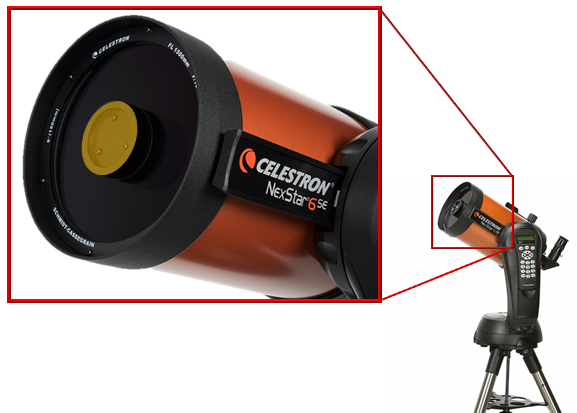
\includegraphics[width=9cm]{images/c03/Cassegrain-Obstruction.png}
    \caption{A Schmidt-Cassegrain telescope with its central obstruction highlighted in light yellow \protect\cite{Schmidt-Cassegrain_Pics}.}
    \label{fig:intro-schmidt-cassegrain}
\end{figure}

At first, it may not seem like central obstruction could be harmful to OAM beams because of their, also central, phase singularity expressed as a dark region. However, as this work will show later, OAM beams not only are not immune to this obstruction, but also can suffer from very destructive changes in their phase. Interestingly enough, there are other type of OAM beams, called perfect vortices, which distinguish themselves from the regular ones in that they don't grow as they propagate, or at least, not as much. This work will also demonstrate that perfect vortices are considerably more resistant to deformation than regular vortices, therefore making them a better candidate for FSO links using Schmidt-Cassegrain telescopes. These types of vortices are as easy to realize as regular ones, which makes them an excellent alternative to enhance the stability of optical telecommunication link.

%====================================================================================================
\section{Motivation}
\label{c1:Motivation}

FSO links are a promising technology as they could potentially enhance both speed and privacy, compared to currently implemented systems. Compared to fiber optics, an FSO could be up to 31\% faster, approaching light speed, thanks to air having a smaller refractive index than glass (for details on the demonstration, please refer to appendices \ref{FiberOptics} and \ref{LightSpeed_FiberOptics}). This difference is even larger when comparing them to copper wires (like coaxial), where the signals travel at lower than 1\% the speed of light. This is without considering additional factors in this material like resistance, electromagnetic interference and thermal dissipation. Multiplexation can also benefit the link's speed by allowing multiple beams to be transmitted in the same channel, as it was explained before; in other words, it could allow more potential users to perceive high speeds simultaneously. Moving on to privacy, third-party eavesdropping on the link could easily be recognized since optical elements are intensity-sensitive to obstacles like lenses, mirrors and also complete blockades.

FSOs are also paramount for inter-satellite communications. Currently, SpaceX is putting into orbit a satellite network capable of providing internet to remote locations, called Starlink. Their objective is to match the speed and latency of an Earth-based internet service provider using copper wires or optical fiber. In order to do so, SpaceX is relying on over 5,000 satellites interconnected by laser FSO links. Here, the reliability of the link is crucial for the wrongful decoding or reception between any two satellites could jeopardize the network's stability, and therefore, usability. Since there is no atmospheric turbulence in outer space, the larger risk in this scenario are the possible deformations that the telescopes' lenses can exert on the beams.

In summary, because FSOs provide crucial benefits over the existent technologies, they are becoming more crucial everyday and for near-future links for the communication's backbone of our civilization. For this reason, it is of the most utter relevance to research and produce products that can add to their reliability and help them achieve their potential.

%====================================================================================================
\section{Objectives}
\label{c1:Objectives}
The main objective of this work is to determine if either regular or perfect vortices suffer from deformations that could render them unusable on a link that presents central obstructions. The following list is a set of steps required to simulate, examine and corroborate this.

\begin{itemize}
  \item Create regular and perfect vortices with obstructions through MATLAB simulations.
  \item Take their intensity profiles to search for compromises in the OAM ``structure'' (this is, preservation of its phase singularity).
  \item Measure their topological charge by taking a circular profile of the OAM's phase subsequent to its propagation.
  \item Compare the OAM's between each other and an unobstructed copy of themselves under the same propagation distance.
\end{itemize}

By doing the previous steps, one should be able to determine if a vortex has been deformed beyond repair. The profiles bring a qualitative analysis that is easier to see and more accurate than examining the vortex's phase and intensity in their entirety. The intensity profile can reveal integral degradation to the OAM structure, while the phase one yields a plot that can help to determine the apparent topological charge of the propagated field with respect to the same unobstructed field. 

%\section{Methodology}
%\label{c1:Methodology}
%To verify the main objective, the scenario was simulated in MATLAB, with the help of pre-existent scripts to create the regular and perfect vortices' phase masks and the basic mathematical model of propagation. New scripts were created to simulate the obstructions, propagate the obstructed beams and take their intensity and phase profiles, in obedience of the steps presented in the previous section.

%First, the necessary scripts that create both types' phase masks along with a different script to model near and far field propagation were provided by my thesis advisor, Gustavo Funes, and Herbert Bravo, UANDES alumni whose thesis' work was to create perfect vortices, who was also under Funes' tutorship.

%Secondly, a propagation script was created using the pre-existent models, and adding arguments that enabled modifications to the scenario like staged propagation and correct automatic identification of the use of either near or far field models.

%Then, the obstruction script was created. This simply added an arbitrary sized black circle at the center of the mask, to represent the obstruction. This script was created keeping in mind that obstruction may not appear at the very beginning of the propagation, but at any intermediate position.
    % Introducción

\chapter{Framework} 
\label{Framework} % la etiqueta para referencias

%En los capitulos no usar mas de un nivel de subtitulos, i.e. subsection.
\section{Light as an Electromagnetic Wave} 
\label{Light is an EM Wave}

To understand how optical vortices work, and how they can be manipulated, first one must understand how light's behavior as an electromagnetic wave, or EM for short; it is important to emphasize that when talking about light, we are usually referring to a light beam. Light's propagation through space, as any other EM wave, can be modeled by equation (\ref{Light Equation}). For the purposes of this paper, phasor notation is preferred as it is useful to distinguish the light beam's real part ($A_0$ in the equation, and also referred to as \textit{intensity} or \textit{intensity field}) from its complex part ($\varphi_0$ in the equation, and also referred to as \textit{phase} or \textit{complex field}).

\begin{equation}
    U_0(r) = A_0e^{i\varphi}
    \label{Light Equation}
\end{equation}

This mathematical representation is mainly supported on Maxwell's four equations, or laws, \cite{Hecht_Optics-Appendix1}.

\begin{equation}
    \nabla \bigcdot \overrightarrow{\textbf{E}} = \frac{\rho}{\epsilon}
    \label{Gauss' Law for Electric Fields}
\end{equation}
\begin{equation}
    \nabla \bigcdot \overrightarrow{\textbf{B}} = 0
    \label{Gauss' Law for Magnetic Fields}
\end{equation}
\begin{equation}
    \nabla \times \overrightarrow{\textbf{E}} = -\frac{\partial \overrightarrow{\textbf{B}}}{\partial t}
    \label{Faraday's Law}
\end{equation}
\begin{equation}
    \nabla \times \overrightarrow{\textbf{B}} = \mu\sigma\overrightarrow{\textbf{E}}+\mu\epsilon\frac{\partial\overrightarrow{\textbf{E}}}{\partial t}
    \label{Ampere's Law}
\end{equation}

These laws unify the three great concepts of physics: electricity, magnetism and light; in particular, that light is an EM wave\footnotemark. In consequence, to comprehend how light propagates, we must understand what a wave is, and how it propagates. 

\footnotetext{Published by James Clerk Maxwell in 1865 in his work ``A Dynamical Theory of the electromagnetic Field'', where he added a term to Ampère's equation that had been published in 1861 ``On Physical Lines of Force'' which provided consistency with the other laws regarding dynamic fields, and added: ``The agreement of the results seem to show that light and magnetism are affections of the same substance, and that light is an electromagnetic disturbance propagated through the field according to electromagnetic laws''.}

In order to reach the model proposed in equation (\ref{Light Equation}), the concepts of \textit{wave} and \textit{field} and the \textit{wave equation} will be introduced, and alongside with them, the necessary conditions that must be met.

A wave is a spatial disturbance in a medium that carries energy and momentum. There are two\footnotemark{} main types of wave: mechanical and electromagnetic. Their difference lies in that mechanical waves require a physical medium for them to be propagated, while EM waves do not.

\footnotetext{There are other, much less common types of waves, like gravitational waves, plasma waves and quantum waves. The latter are very similar to mechanical waves, but instead follow the principles of quantum physics.}

A field, whether it is electric or magnetic, is a volume that depends on space and time, and can be ``constructed'' upon the variations of position that an arbitrary point within a wave experiences on each spatial axis $(x,y,z)$ as the wave travels. These displacements, which we will name $u(x,t)$, $u(y,t)$ and $u(z,t)$ respectively for each axis, are scalar functions that compose the field $\overrightarrow{\textbf{U}}(R,t)$, where $R = (x,y,z)$. The wave's dependencies on space and time exist because 1) it occupies a position in a volume or \textit{space} that 2) varies in time as it travels.

A simple illustration of this phenomenon can be seen in figure (\ref{fig:u_parameter_explanation}). Here, a mechanical wave is seen as it travels through a rope. The arbitrary point could be located anywhere within the rope, for example, at its center. The displacement this point will experience can be traced and then plotted. Naturally, the ``shape'' of the reference point's displacement should be wave-like, with respect to time. 

\begin{figure}[htbp]
    \centering
    \fbox{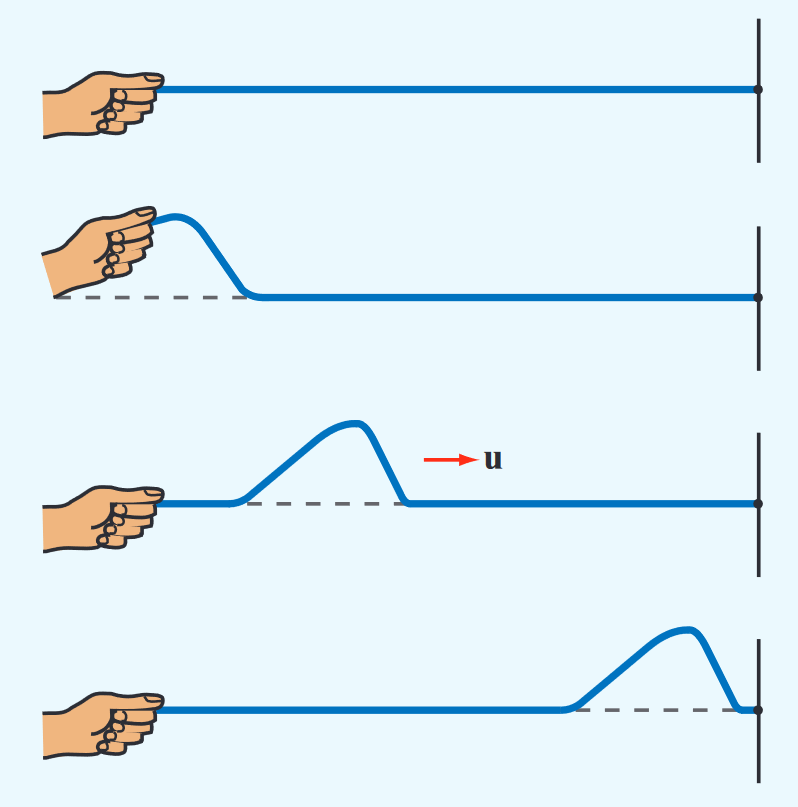
\includegraphics[width=8cm, height = 5.5cm]{images/c02/EM Waves/Wave_u_parameter.PNG}}
    \caption{Displacement $u$ of an arbitrary point as a wave travels through a rope in space and time \cite{u_parameter_explanation-figure}.}
    \label{fig:u_parameter_explanation}
\end{figure}

The wave equation describes this relationship better, and can be deduced from Ampère and Faraday's laws (refer to appendix \ref{WaveEquation_MaxwellEquations} for the mathematical demonstration). It describes the propagation of an EM wave through a medium, including vacuum.

\begin{equation}
    \nabla^2 \overrightarrow{\textbf{U}} = \frac{1}{c_0^2}\frac{\partial^2 \overrightarrow{\textbf{U}}}{\partial t^2}
    \label{Wave_Equation}
\end{equation}

Where $\overrightarrow{\textbf{U}}$ is the field\footnote{It could be either the electric field $\overrightarrow{\textbf{E}}$ or magnetic $\overrightarrow{\textbf{B}}$.}, $c_0$ is the propagation speed of the wave given by $c_0 = \frac{1}{\sqrt{\mu_0 \epsilon_0}}$, ($\mu_0$ and $\epsilon_0$ are the magnetic and electric permeability constants of the medium, respectively) and $t$ is time. Light in vacuum travels, naturally, at the speed of light, a number represented by the letter $c$ and equal to 299,792.458 $[\frac{km}{s}]$ (185,871,323.96 $[\frac{mi}{s}]$\footnote{NIST approximates a mile as $0.62 \times km$}) \cite{Hecht_Optics-Chapter3_EM_Waves} \cite{Speed_of_Light:NIST}.

Do note that the Laplacian is noted by the symbol $\nabla$ (read \textit{nabla}) and it represents the curl of the tridimensional field. It summarizes that the operation is being carried out in each spatial axis.

\begin{equation}
    \nabla^2 \overrightarrow{\textbf{U}} = \frac{\partial^2 \overrightarrow{\textbf{U}}}{\partial x^2} + \frac{\partial^2 \overrightarrow{\textbf{U}}}{\partial y^2} + \frac{\partial^2 \overrightarrow{\textbf{U}}}{\partial z^2}
    \label{Laplacian}
\end{equation}

Then, by rewriting equation (\ref{Wave_Equation}) in terms of equation (\ref{Laplacian}), the following equation results.

\begin{equation}
    \frac{\partial^2 \overrightarrow{\textbf{U}}}{\partial x^2} + \frac{\partial^2 \overrightarrow{\textbf{U}}}{\partial y^2} + \frac{\partial^2 \overrightarrow{\textbf{U}}}{\partial z^2} = \frac{1}{c_0^2}\frac{\partial^2 \overrightarrow{\textbf{U}}}{\partial t^2}
    \label{Wave_Equation_Long}
\end{equation}

This equation shows that waves move in the same way of its shape, this means, in a sinusoidal motion. As it was stated before, if we were to plot the displacements of an arbitrary point in the field (left side of \ref{Wave_Equation_Long}), it would have the same shape as the wave itself (right side of \ref{Wave_Equation_Long}), corrected by the inverse of its speed to correctly match the magnitude as well. As for its direction, the symmetry described by Maxwell's equations denote that the disturbance will propagate in a direction that is symmetrical to both the electric $\overrightarrow{\textbf{E}}$ and magnetic $\overrightarrow{\textbf{B}}$ fields. Waves that propagate in this manner are called transverse waves, and is the case for all EM waves, light included. 

%What this equation is telling us is that the wave propagates with a profile resembling the one of the wave. In other words, the shape that it takes during the propagation (right side of \ref{Wave_Equation_Long}) is directly related with the wave's shape (left side of \ref{Wave_Equation_Long}), corrected by the inverse of its speed. As for its direction, the symmetry imposed by Maxwell's equations denote that the disturbance will propagate in a direction that is symmetrical to both the electric $\overrightarrow{\textbf{E}}$ and magnetic $\overrightarrow{\textbf{B}}$ fields. Waves that propagate in this manner are called transverse electromagnetic waves, or TEM for short.

\begin{figure}[htbp]
    \centering
    \fbox{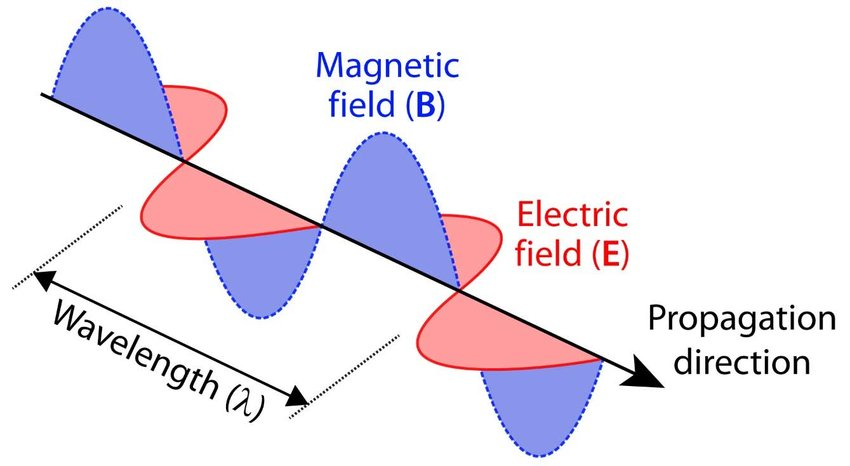
\includegraphics[scale=0.45]{images/c02/EM Waves/Light_EM_Wave.png}}
    \caption{Representation of a light wave propagating through space showing both of its fields, its wavelength ($\lambda$) and direction (black arrow) \cite{Light_EM_Wave_Figure}. Its direction is given by the cross-product $\overrightarrow{\textbf{E}} \times \overrightarrow{\textbf{B}}$.}
    \label{fig:Light_EM_Wave}
\end{figure}

%Light is created from the thermonuclear reactions inside our Sun, as a consequence of the collision between hydrogen atoms, which in turn produce helium atoms. Moreover, light is one form of released energy from the an electron's shift between energy levels (either by yielding or receiving energy) within an atom; in other words, part of the energy differential is released in the form of photons\footnotetext{Other energy forms irradiated by the Sun are radiation, mainly ultraviolet and solar winds.}. These photons are known as the light particles, and they vibrate at different frequencies. 

Classical physics tell us that in all waves, frequency and wavelength are related by equation $\lambda = \frac{c_0}{f}$, where $f$ is the wave's frequency, $c_0$ it's speed and $\lambda$ it's wavelength. EM waves can have different wavelengths, or alternatively, frequencies, that can be seen in figure (\ref{fig:EM_Spectrum}). We humans perceive a portion of these wavelengths in the form of colors that compose the \textit{visible spectrum} of light. According to Hecht, ``light corresponds to the EM radiation in the narrow band from about $3.84 \times 10^{14}$ Hz to roughly $7.69 \times 10^{14}$ Hz'' \cite{Hecht_Optics-Visible_Light}. Some examples of colors and their respective wavelength and frequency, can be seen in table (\ref{tab:VisibleLight}).

\begin{figure}[htbp]
    \centering
    \fbox{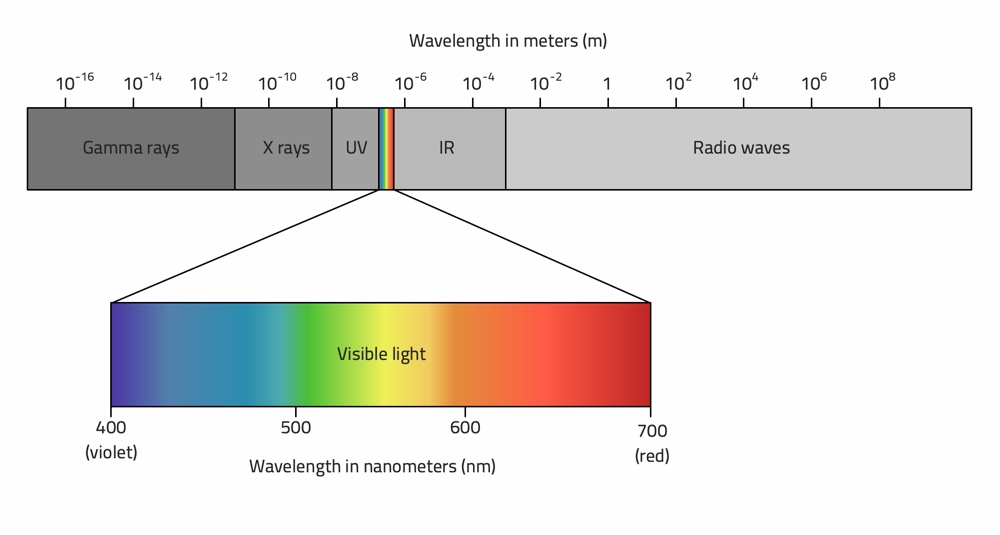
\includegraphics[width=11cm]{images/c02/EM Waves/EM_Spectrum.jpg}}
    \caption{EM Spectrum \cite{EM_Spectrum-Figure}. The visible spectrum is encompassed between 390 and 780 [nm] although it is usually approximated to the range 400-700 [nm].}
    \label{fig:EM_Spectrum}
\end{figure}

\begin{table}[htbp]
    \centering
    \begin{tabular}{|l|c|c|}
    \hline
    \textbf{Color} & \textbf{$\lambda_0$ [nm]} & \textbf{$f$ [HZ]} \\ \hline
    Red           & 780-622                       & 384-482                  \\ \hline
    Orange        & 622-597                       & 482-503                  \\ \hline
    Yellow       & 597-577                       & 503-520                  \\ \hline
    Green          & 577-492                       & 520-610                  \\ \hline
    Blue           & 492-455                       & 610-659                  \\ \hline
    Violet        & 455-390                       & 659-769                  \\ \hline
    \end{tabular}
    \caption{Wavelength, in nanometers, and frequency, in terahertz, for some colors of the visible spectrum \cite{Hecht_Optics-Visible_Light}. There is no international standard regarding the accuracy of these ranges are, as some variations of the upper and lower limits of the visible spectrum vary within the tens of nanometers.}
    \label{tab:VisibleLight}
\end{table}

\newpage
It is useful to distinguish what we perceive as light, as what might seem as a source of unique color, can actually be made out of multiple ones. For instance, sources like our Sun or a light bulb produce white light\footnote{The Sun looks yellow from Earth because of the scattering effect that our blue atmosphere has on ``rejecting'' blue and violet waves. However, this can be an extensive topic, worthy of its own.}, which is a combination of all colors, or wavelengths. On the other hand, monochromatic light are waves that share the same wavelength; for example, laser light is monochromatic. Therefore, in essence, although light can appear to be made out of multiple-frequency-waves, a single light wave is monochromatic.

\begin{figure}[htbp]
    \centering
    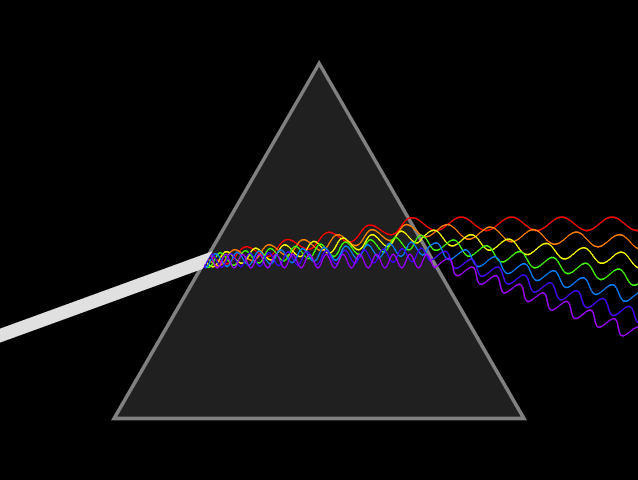
\includegraphics[width=6cm]{images/c02/EM Waves/Prism.PNG}
    \caption{Chromatic dispersion in a prism as a white light beam enters it. Sir Isaac Newton discovered that a sunbeam impinging on a prism at a certain angle can disperse the colors ``contained'' in this beam and show them separately in the late XVII century.}
    \label{fig:Prism}
\end{figure}

%Now that we have established some of light's properties and its behavior as an EM wave, we can continue with our demonstration.

Using this information to move on to our demonstration, we can notice that because light is a wave, a solution to its wave equation (\ref{Wave_Equation}) is another wave. Hence, the solutions we are looking for have the form of equation (\ref{Wave_Equation_Cartesian_Solution}).

%Como una única onda de luz es monocromática, las variaciones de campo que experimenta son sinusoidales, puesto que una solución a la ecuación de onda (\ref{Wave_Equation}) es la misma onda, multiplicada por el inverso de su velocidad al cuadrado, en este caso $c$ (o unos 90 kilómetros por segundos menos que $c$ dentro de la Tierra). En otras palabras, las soluciones son de la forma:

\begin{equation}
    U_0(r) = A_0\cos(\omega t + kr)
    \label{Wave_Equation_Cartesian_Solution}
\end{equation}

Where $A_0$ is the amplitude, given by $A_0 = A/r$, and $r = x^2 + y^2 + z^2$, $\phi = kr$ its phase and $k = \frac{2\pi}{\lambda} = \frac{\omega}{c_0}$. Finally, this equation can be rewritten as a phasor, which looks like our target equation (\ref{Light Equation}).

\begin{equation}
    U_0(r) = A_0e^{i\phi}
\end{equation}

%Nótese que la dependencia de la ecuación cambia de $R$ a $r$ si se asumen dos cosas. La primera es que, si bien para poder determinar la posición de una onda precisamos del tiempo, la misma onda puede ser generada en cualquier instante de tiempo. Por ejemplo, si se prende y apaga una fuente de luz, como una ampolleta o láser, en dos momentos distintos (por ejemplo, en días diferentes) la luz emitida por estas fuentes tienen el mismo comportamiento en ambos casos. De esta forma, la forma y comportamiento no dependen directamente del tiempo. La segunda es que, dado que el comportamiento no depende del tiempo, se puede fijar de la misma forma uno de los tres ejes sobre el cual la onda siempre se propaga. Convenientemente, este eje puede ser el eje óptico, que es el resultado de pensar en la propagación de la onda desde el plano en $R$ dado por $z = 0$. De esta forma, se puede reducir la ecuación de onda independientemente del tiempo, y redefiniendo $z$ como la distancia de propagación de la onda desde la fuente o instante de tiempo dados.

%\section{Polarización}
%\label{c2:Polarization}

%The beams used for traditional optical communications are not simple lasers being transmitted, on and off, through an optical fiber. Instead, they are special shapes achieved by inducing momentum on simple beams. However, before jumping to how this momentum is induced, knowing the types of polarization can ease the way towards understanding why light behaves how it does under these special forces 

%Para poder entender las formas en que la luz puede expresar momento, es útil entender un poco del fenómeno de la polarización.

%La polarización de una onda EM es la orientación, expresada como el ángulo del campo eléctrico ($\overrightarrow{\textbf{E}}$) con respecto a un eje de referencia cuyo orígen coincide con el del eje óptico ($z$).

%\begin{figure}[htbp]
%    \centering
%    \fbox{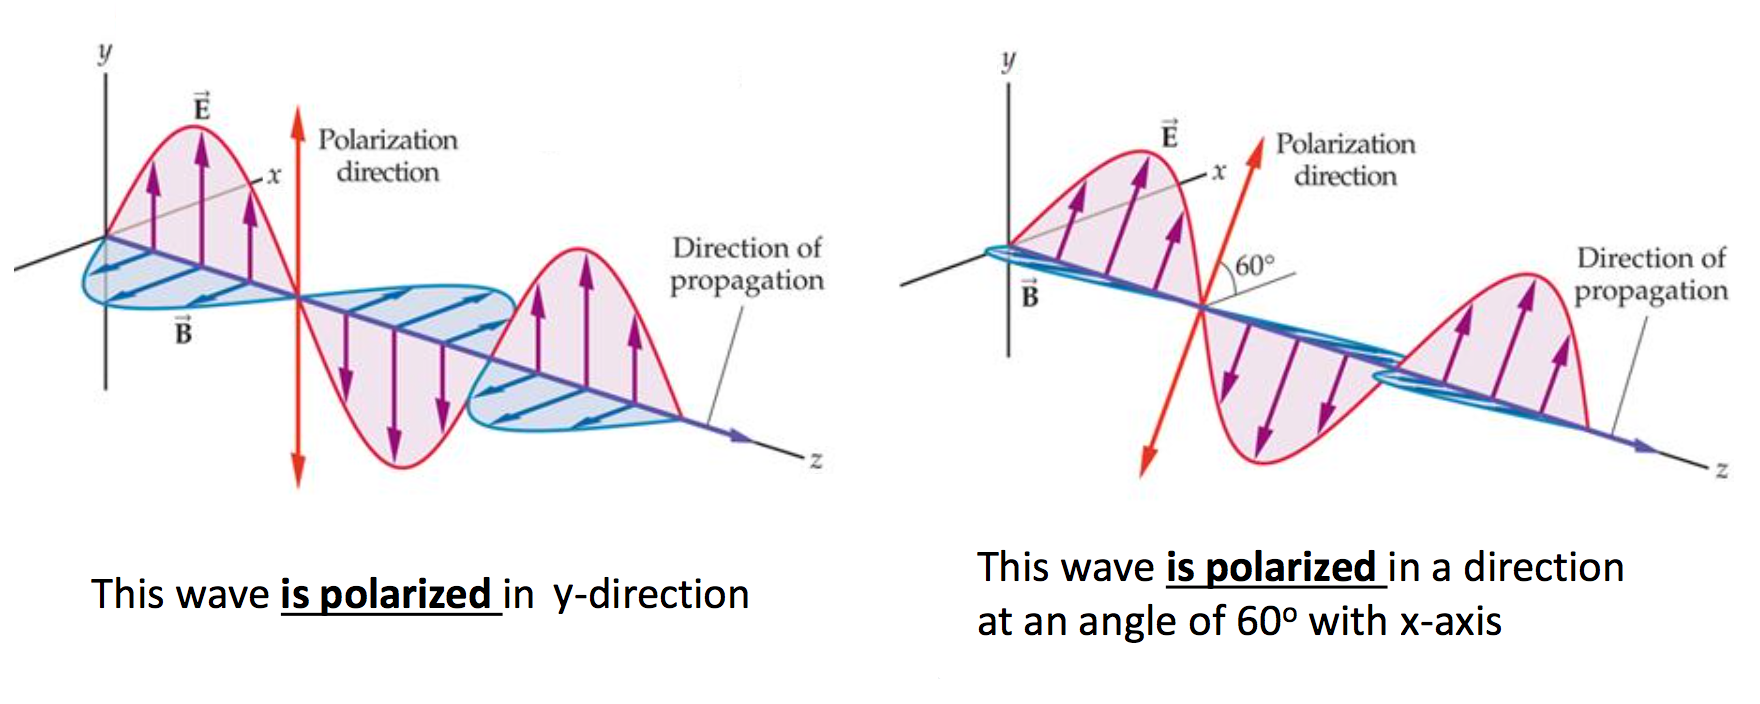
\includegraphics[width=12cm]{images/c02/Polarization/Linearly_Polarized_Light.png}}
%    \caption{Ilustración de polarización lineal.}
%    \label{fig:Linear_Polarization}
%\end{figure}

%Existen tres tipos de polarización: lineal, circular y elíptica (Véase figura \ref{fig:Types_of_Polarization}). Adicionalmente, existe la luz no polarizada, que consiste de varias ondas con distintas polarizaciones, por lo que el conjunto no tiene una definida. Un ejemplo de luz no polarizada es la luz blanca (Véase figura \ref{fig:Unpolarized_Light}), aquella irradiada por el sol o una ampolleta, que contiene varias ondas a distintas polarizaciones y longitudes de onda. 

%\begin{figure}[htbp]
%    \centering
%    \fbox{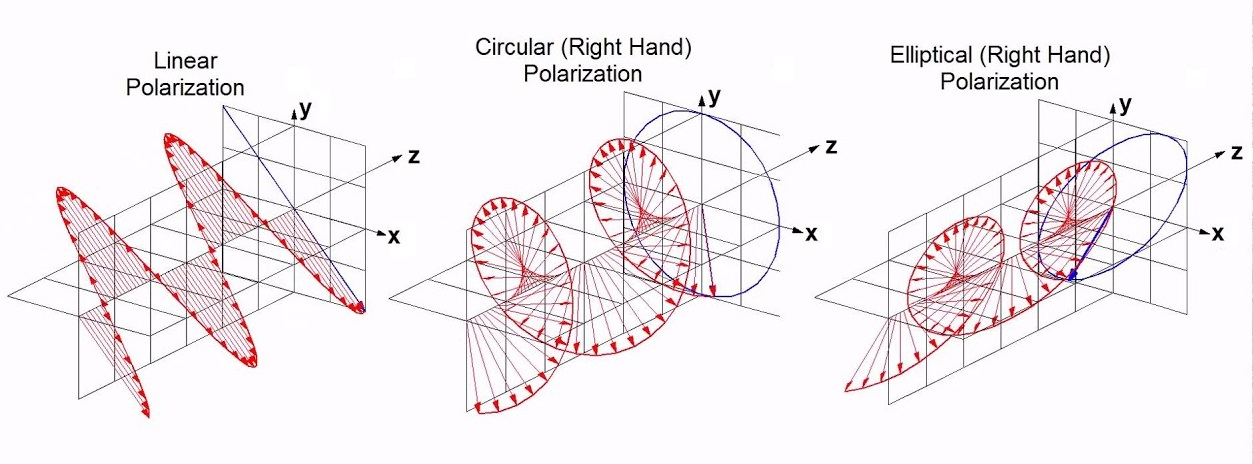
\includegraphics[width=12cm]{images/c02/Polarization/Types_of_Polarization.jpg}}
%    \caption{Tipos de polarización: lineal (izquierda), circular (centro) y elíptica (derecha). En esta ilustración se obvia, por simplicidad, el campo electromagnético $\overrightarrow{\textbf{B}}$, que es perpendicular al campo eléctrico $\overrightarrow{\textbf{E}}$, ilustrado en rojo \cite{Types_of_Polarization_Figure}.}
%    \label{fig:Types_of_Polarization}
%\end{figure}

%\begin{figure}[htbp]
%    \centering
%    \fbox{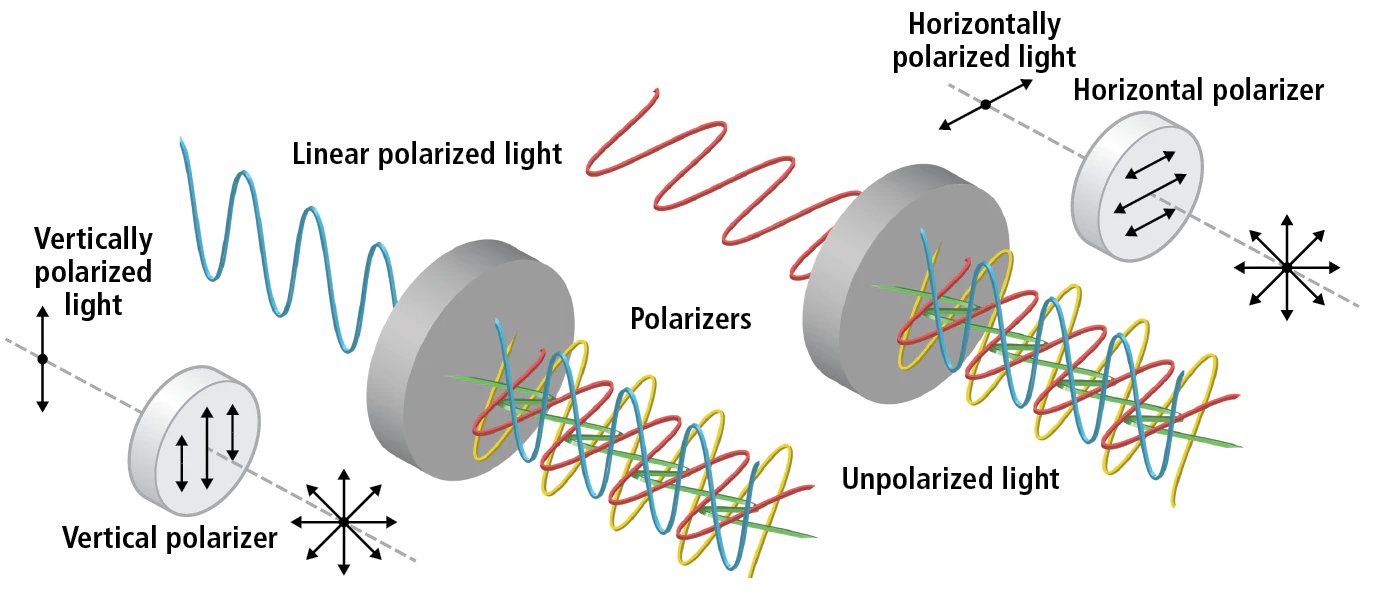
\includegraphics[width=12cm]{images/c02/Polarization/Unpolarized_Light.png}}
%    \caption{Ilustración de luz no polarizada \cite{Unpolarized_Light_Figure}.}
%    \label{fig:Unpolarized_Light}
%\end{figure}

%La polarización, en cualquier caso, se puede entender como el vector resultante de una composición de dos vectores: en $\hat{x}$ y en $\hat{y}$. De esta forma, cualquier tipo de polarización puede ser representada como una función de estas dos componentes, sólo cambiando la magnitud de cada una. Para los casos de la polarización circular y elíptica, las magnitudes varían en el tiempo.

%Ahora, ¿Qué tiene que ver la polarización con el momento de una onda EM? Como bien se dijo en la sección anterior, una onda EM puede transportar momento. Hasta antes del año 1992, se sabía que la luz transporta un momento lineal equivalente a $\hbar k_0$ por fotón, y si está polarizada circularmente, un momento de giro angular (SAM, por sus siglas en inglés derivadas de \textit{Spin Angular Momentum}) de $\pm \hbar$ por fotón. Expresado de otra forma, una onda de luz polarizada linealmente no transporta SAM, pero una onda polarizada circularmente sí.

%\begin{figure}[htbp]
%    \centering
%    \fbox{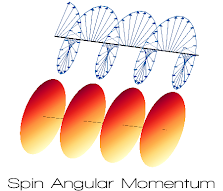
\includegraphics{images/c02/OAM/SAM.png}}
%    \caption{Ilustración de una onda EM polarizada circularmente que posee SAM, mostrando sólo el campo eléctrico, y su visualización espacial.}
%    \label{fig:SAM}
%\end{figure}

\section{Optical vortices with Orbital Angular \\Momentum}
\label{c2:OAM}

In 1992 Allen et. al. published a paper showing that helically phased beams naturally carry an orbital angular momentum (OAM) that is $\ell$ times greater than the spin angular momentum's $\hbar$\footnote{Planck's constant, which is equal to $6.62607015\times 10^{-34}$ $[J\bigcdot s]$.} per photon \cite{Allen_OAM:1992}. Before this discovery, it was known that light can exert momenta upon the surfaces where it bounces off, pushing (linear momentum) or spinning them (spin angular momentum, or SAM). What is more, \textit{linear momentum} carries a momentum of $\hbar k_0$ per photon and, if the light beam is circularly polarized, a SAM of $\pm \hbar$ per photon. Simply put, this publication explained that light can also twist the receiving end \cite{Yao-Padgett:2011}.

Alison Yao and Miles Padgett exemplified these momenta in their work on OAM, to better understand them: ``[...] a laser pointer shone at a door can exert a torque about the hinge, albeit usually not enough to open it! However, when we discuss [OAM] [...] we seek to identify an angular momentum capable of twisting the door knob'' \cite{Yao-Padgett:2011-door_example}.

\begin{figure}[htbp]
    \centering
    \fbox{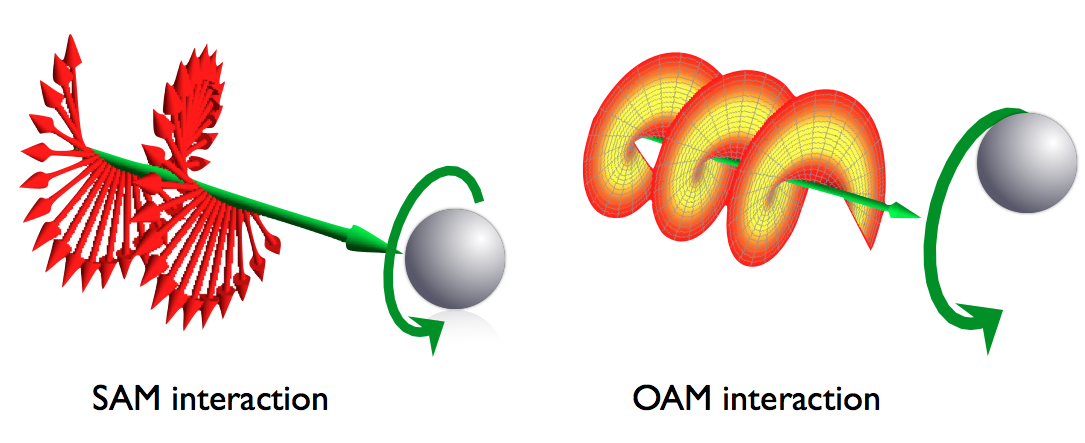
\includegraphics[width=10cm]{images/c02/OAM/SAM_OAM.png}}
    \caption{Comparison between SAM and OAM \cite{Wikimedia:SAM_vs_OAM}}
    \label{fig:SAM_vs_OAM}
\end{figure}

One of the most remarkable features of beams that carry OAM (often referred to as OAM beams) is that they present a phase singularity running along its center that, in turn, is seen as a region of total darkness in intensity. As such, they resemble a vortex, which is defined as a region in a fluid that revolves around an axis line (e.g., water draining in a sink). If we think of light as the ``fluid'', then the beam would be an optical vortex, as its photons revolve around the optical axis. A projected OAM, or vortex, is shown in figure (\ref{fig:Example_OAM}).

%\begin{figure}[htbp]
%    \centering
%    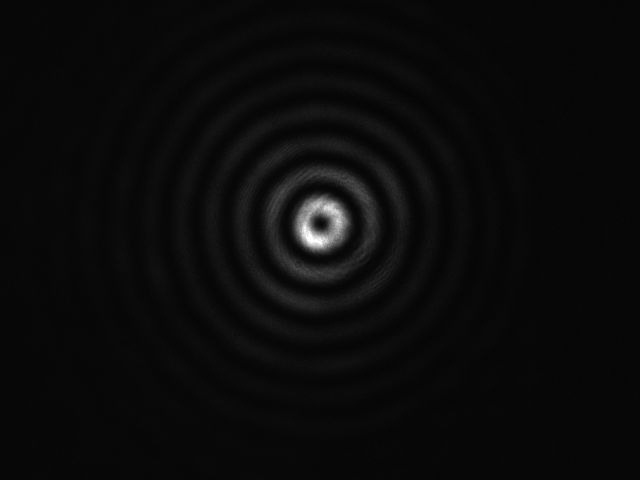
\includegraphics[width=7cm]{images/c02/OAM/OAM.png}
%    \caption{Real regular OAM beam projected onto a surface.}
%    \label{fig:Simple_OAM_Example}
%\end{figure}

\begin{figure}[htbp]
    \centering
    \begin{subfigure}[b]{0.45\textwidth}
        \centering
        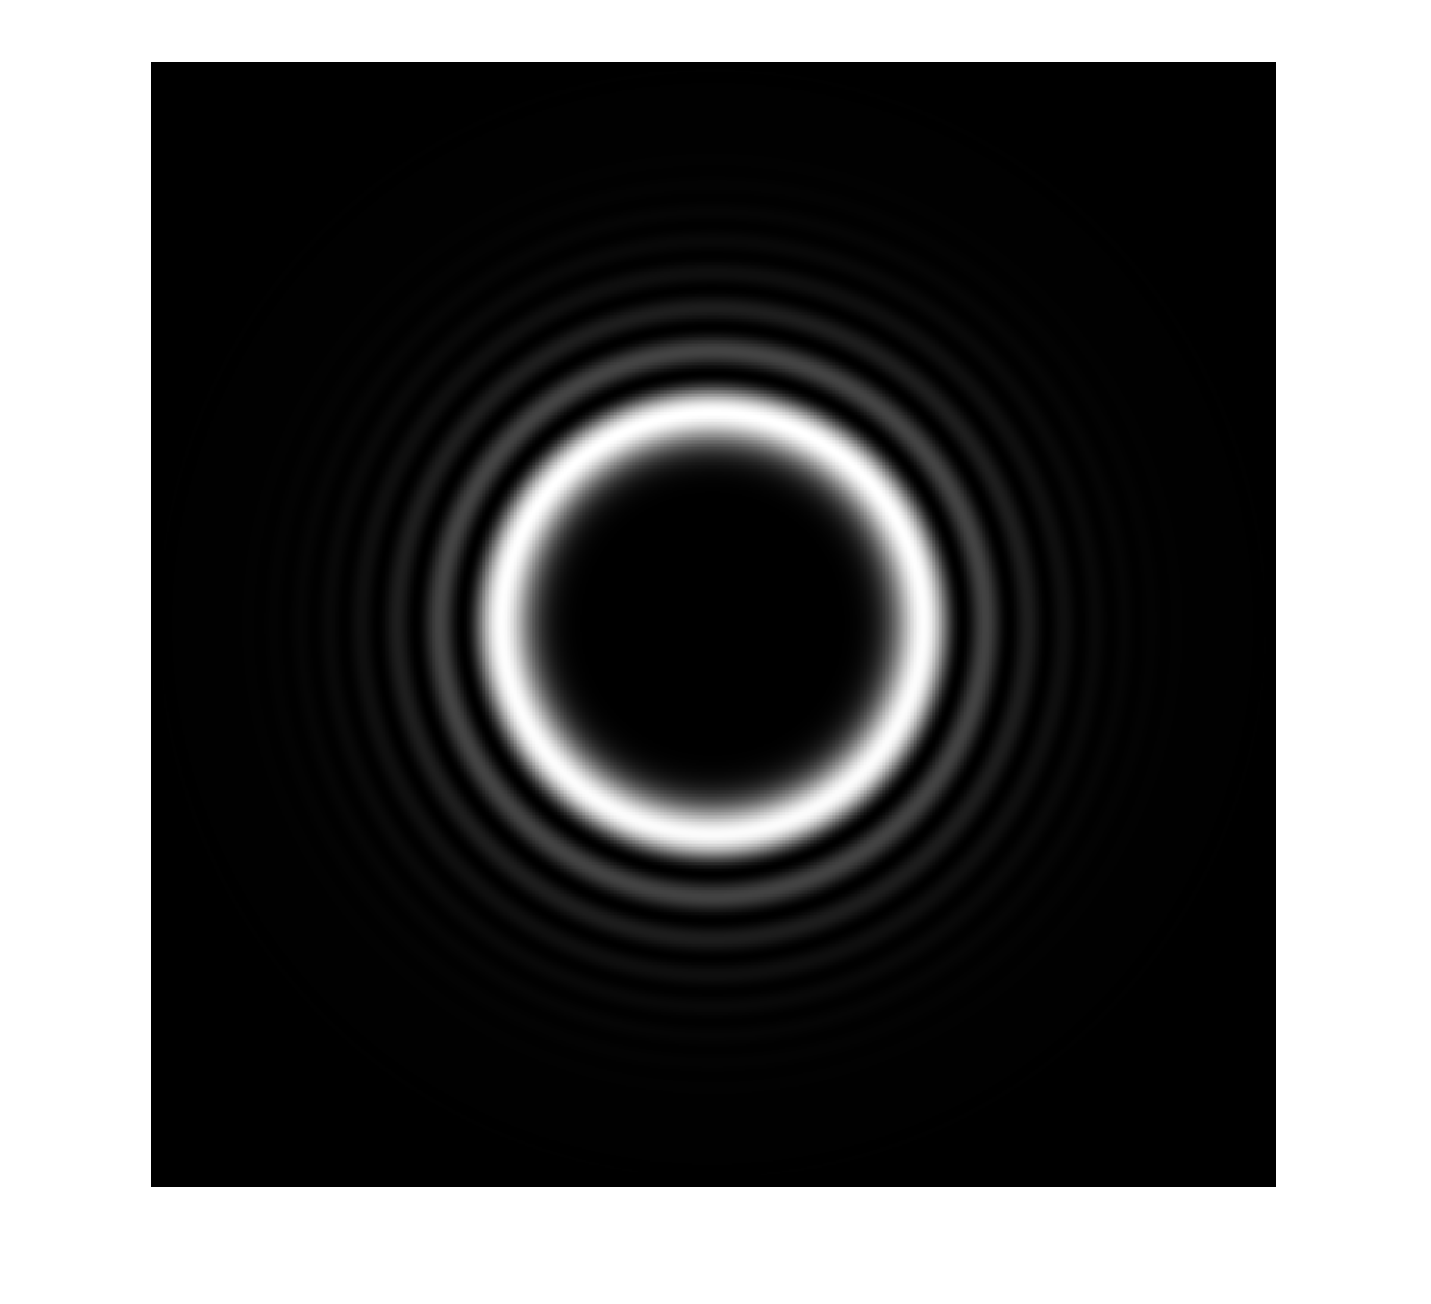
\includegraphics[width=\textwidth]{images/c02/OAM/Regular_OAM.eps}
        \caption{Regular vortex.}
    \end{subfigure}
    \hfill
    \begin{subfigure}[b]{0.45\textwidth}
        \centering
        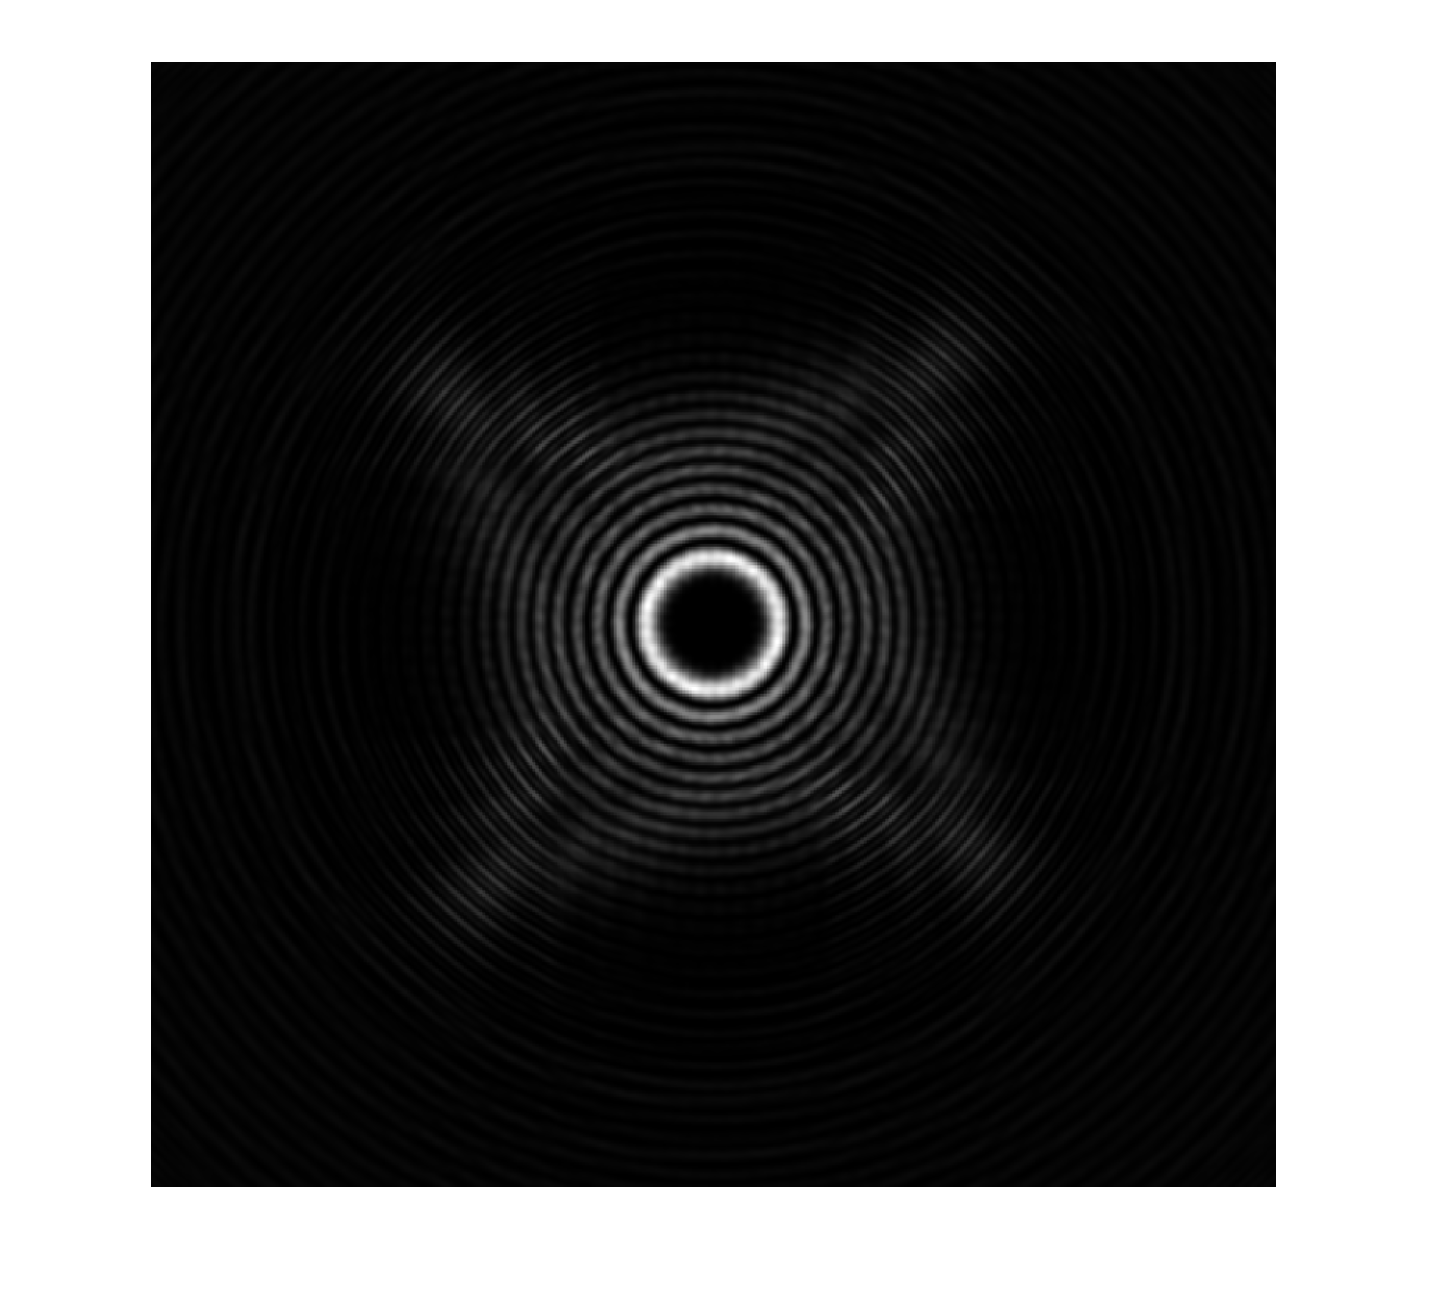
\includegraphics[width=\textwidth]{images/c02/OAM/OAM_10_40.eps}
        \caption{Perfect vortex.}
    \end{subfigure}
    \caption{Optical vortices produced from simulations (Own elaboration).}
    \label{fig:Example_OAM}
\end{figure}

The number $\ell$, the factor that amplifies the momentum of OAM with respect to SAM, is designated \textit{topological charge} or \textit{state}. This number not only translates into the number of ``helices'' the corkscrew-like beam will have, but also correlates to its radial size and, as a consequence, to the size of the phase singularity. A representation of these beams can be seen in figure (\ref{fig:Different_OAM_Beams}). In contrast, \textit{perfect vortices} are a special type whose size, in theory, does not correlate to the state of the OAM; in other words, they are constant in size as they propagate \cite{Thesis_Herbert_PerfectVortices:2020}.

\begin{figure}[htbp]
    \centering
    \fbox{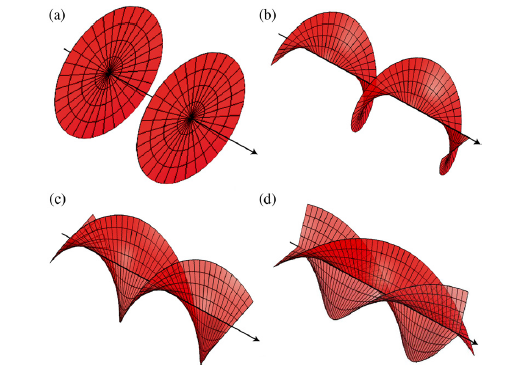
\includegraphics[width=9.5cm]{images/c02/OAM/OAM_topological_charge.PNG}}
    \caption{OAM beams of topological charges: (a) $\ell = 0$, (b) $\ell = 1$, (c) $\ell = 2$ and (d) $\ell = 3$. These illustrations show how OAM states differ from each other, disregarding their projections onto a surface \cite{Yao-Padgett:2011}.}
    \label{fig:Different_OAM_Beams}
\end{figure}

Regular OAM beams tend to grow in size and change in shape as they travel from the source towards infinity. At the very beginning, the beam does not resemble a beam like that of figure (\ref{fig:Example_OAM}), however as the distance $z$ increases, the more it resembles it. The beam will not only take this shape, but will also keep growing in radial size, which also means that its intensity fades away as the region the same light covers grows. As the beam approaches infinity, its shape will be even more static and its growth will also slow significantly. Perfect OAMs also evolve along the propagation distance, yet they don't grow in size. These phenomena will be further explained in section (\ref{c2:Near and Far Field Propagation}).

A feature that both regular and perfect OAM beams share, is their intensity distribution. The lasers commonly used in optics have a Gaussian distribution, that is, very bright at its mean $\mu$ and fades at a rate related to its standard deviation $\sigma$. As figure (\ref{fig:Example_OAM}) shows, OAM beams can have rings. The intensity distribution, following that of a Gaussian, tends to concentrate most of the intensity in the smaller, most centered ring (also referred to as the main ring). The surrounding rings follow a Gaussian distribution, considering the ``skips'' they have between them. This is better illustrated in the following figure.

\begin{figure}[htbp]
    \centering
    \begin{subfigure}[b]{0.45\textwidth}
        \centering
        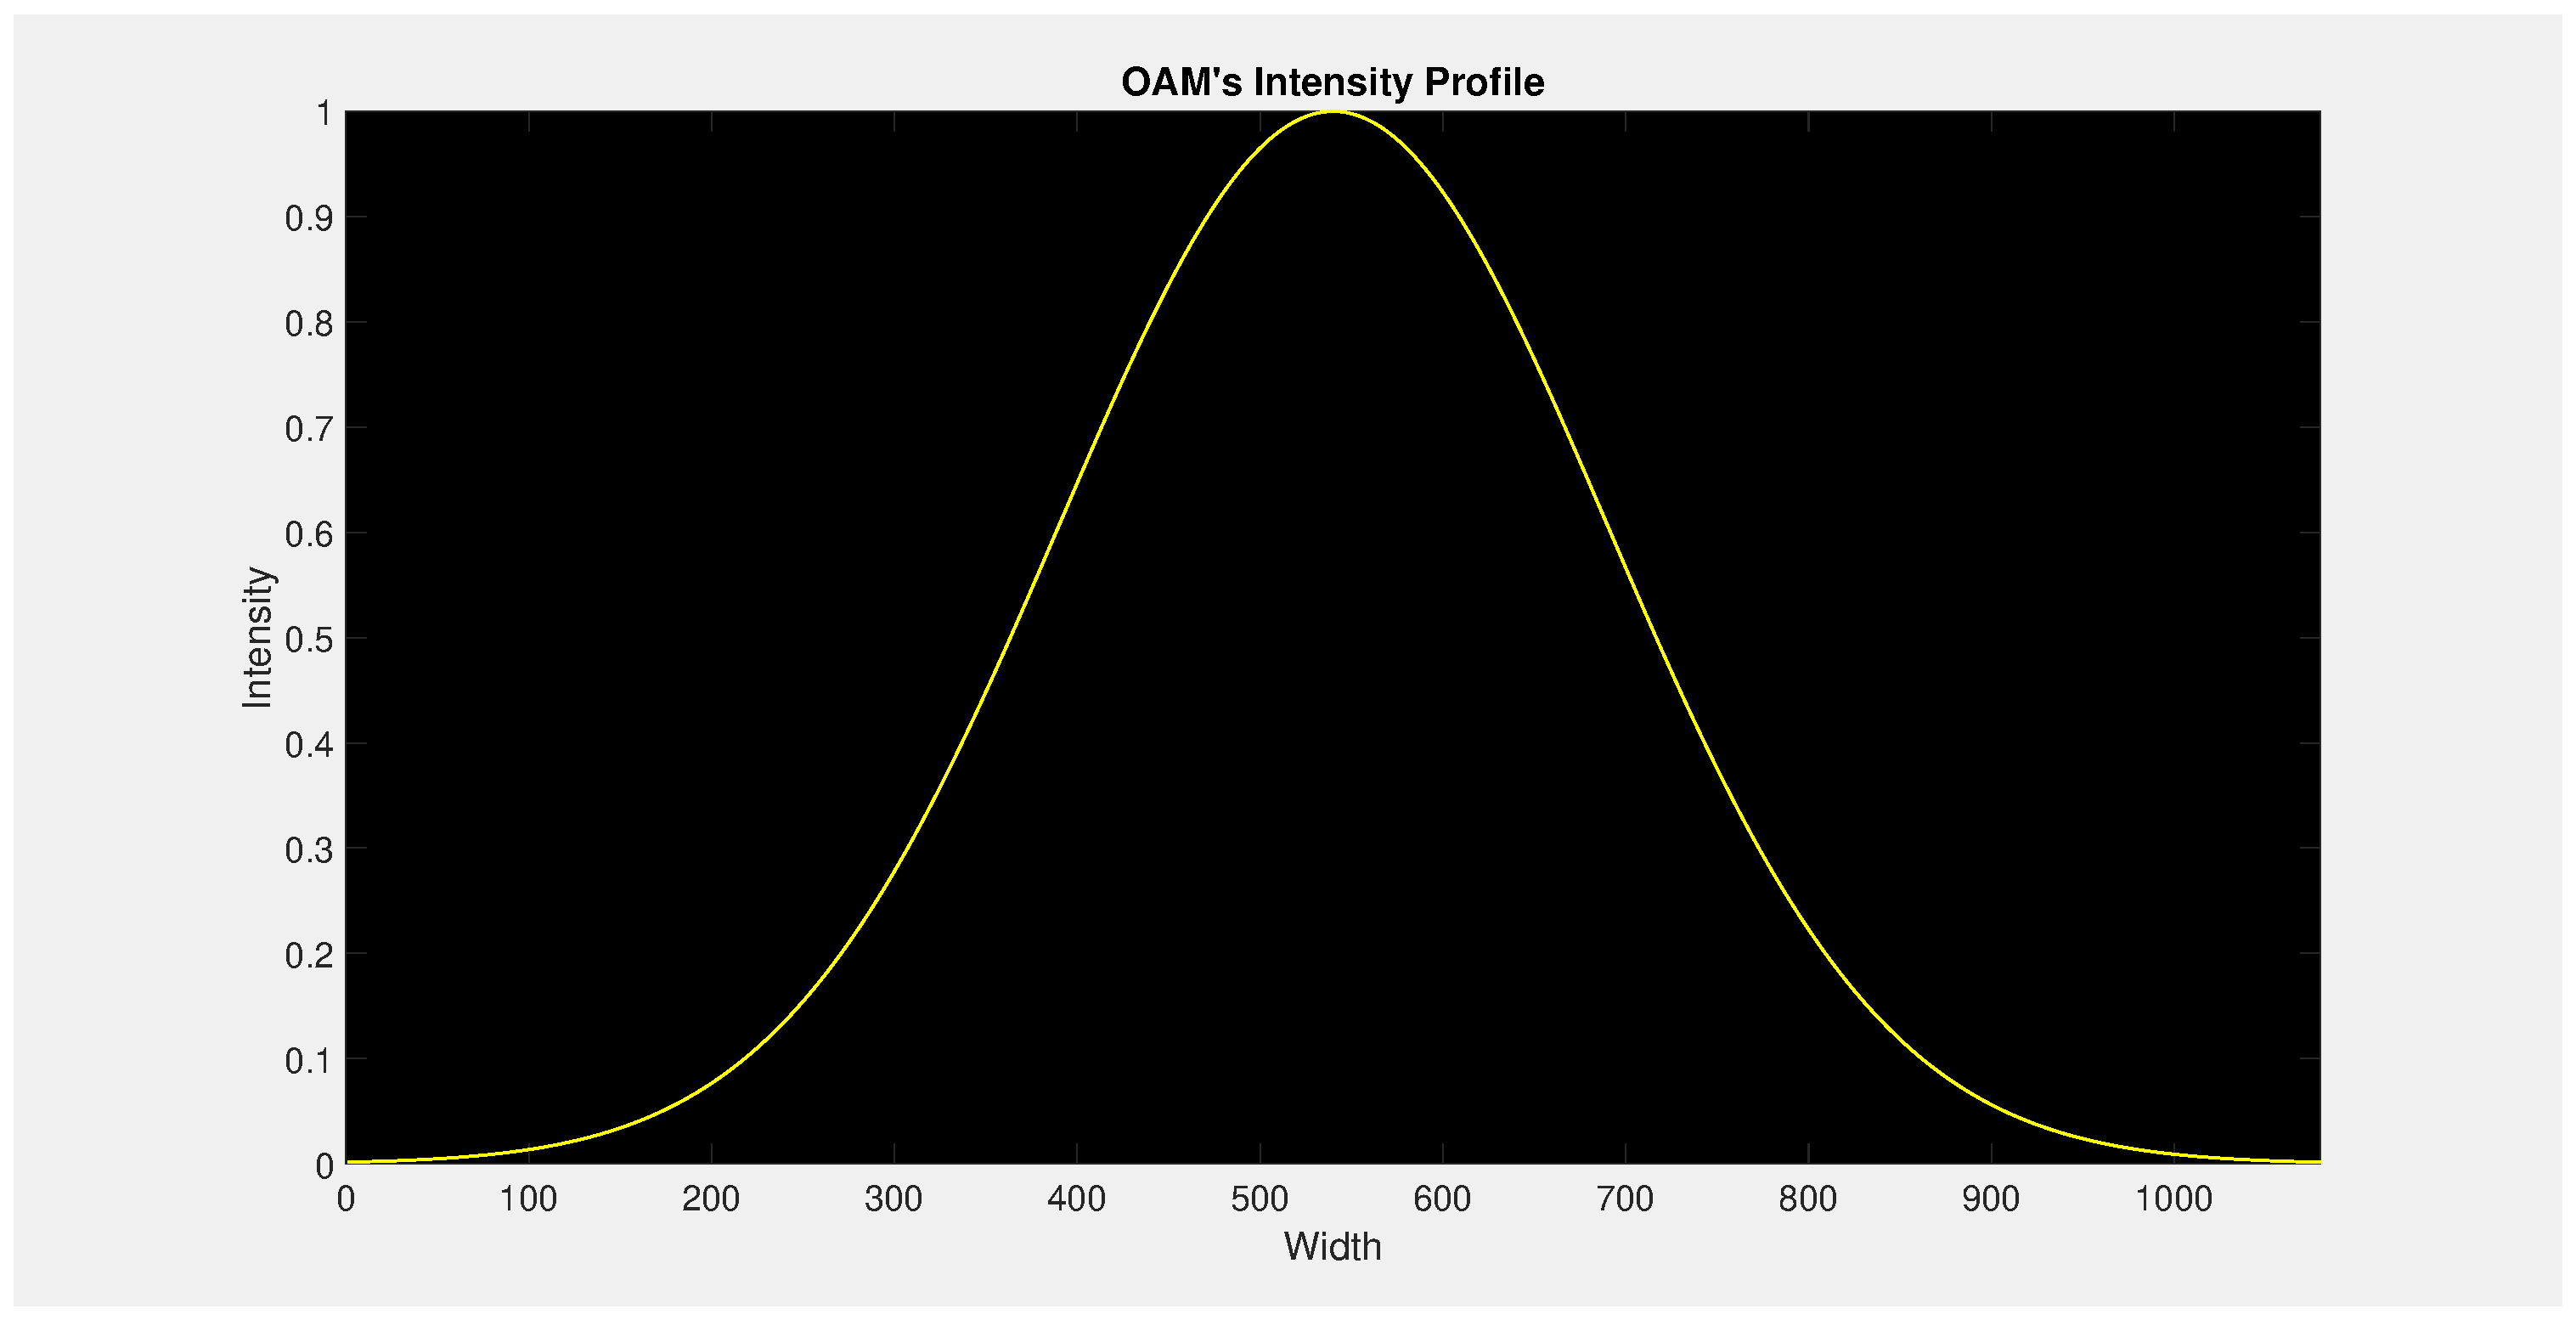
\includegraphics[width=\textwidth]{images/c02/OAM/Gauss_Profile.eps}
        \caption{Regular Gaussian beam's intensity profile.}
        \label{fig:example_Gaussian_profile}
    \end{subfigure}
    \hfill
    \begin{subfigure}[b]{0.45\textwidth}
        \centering
        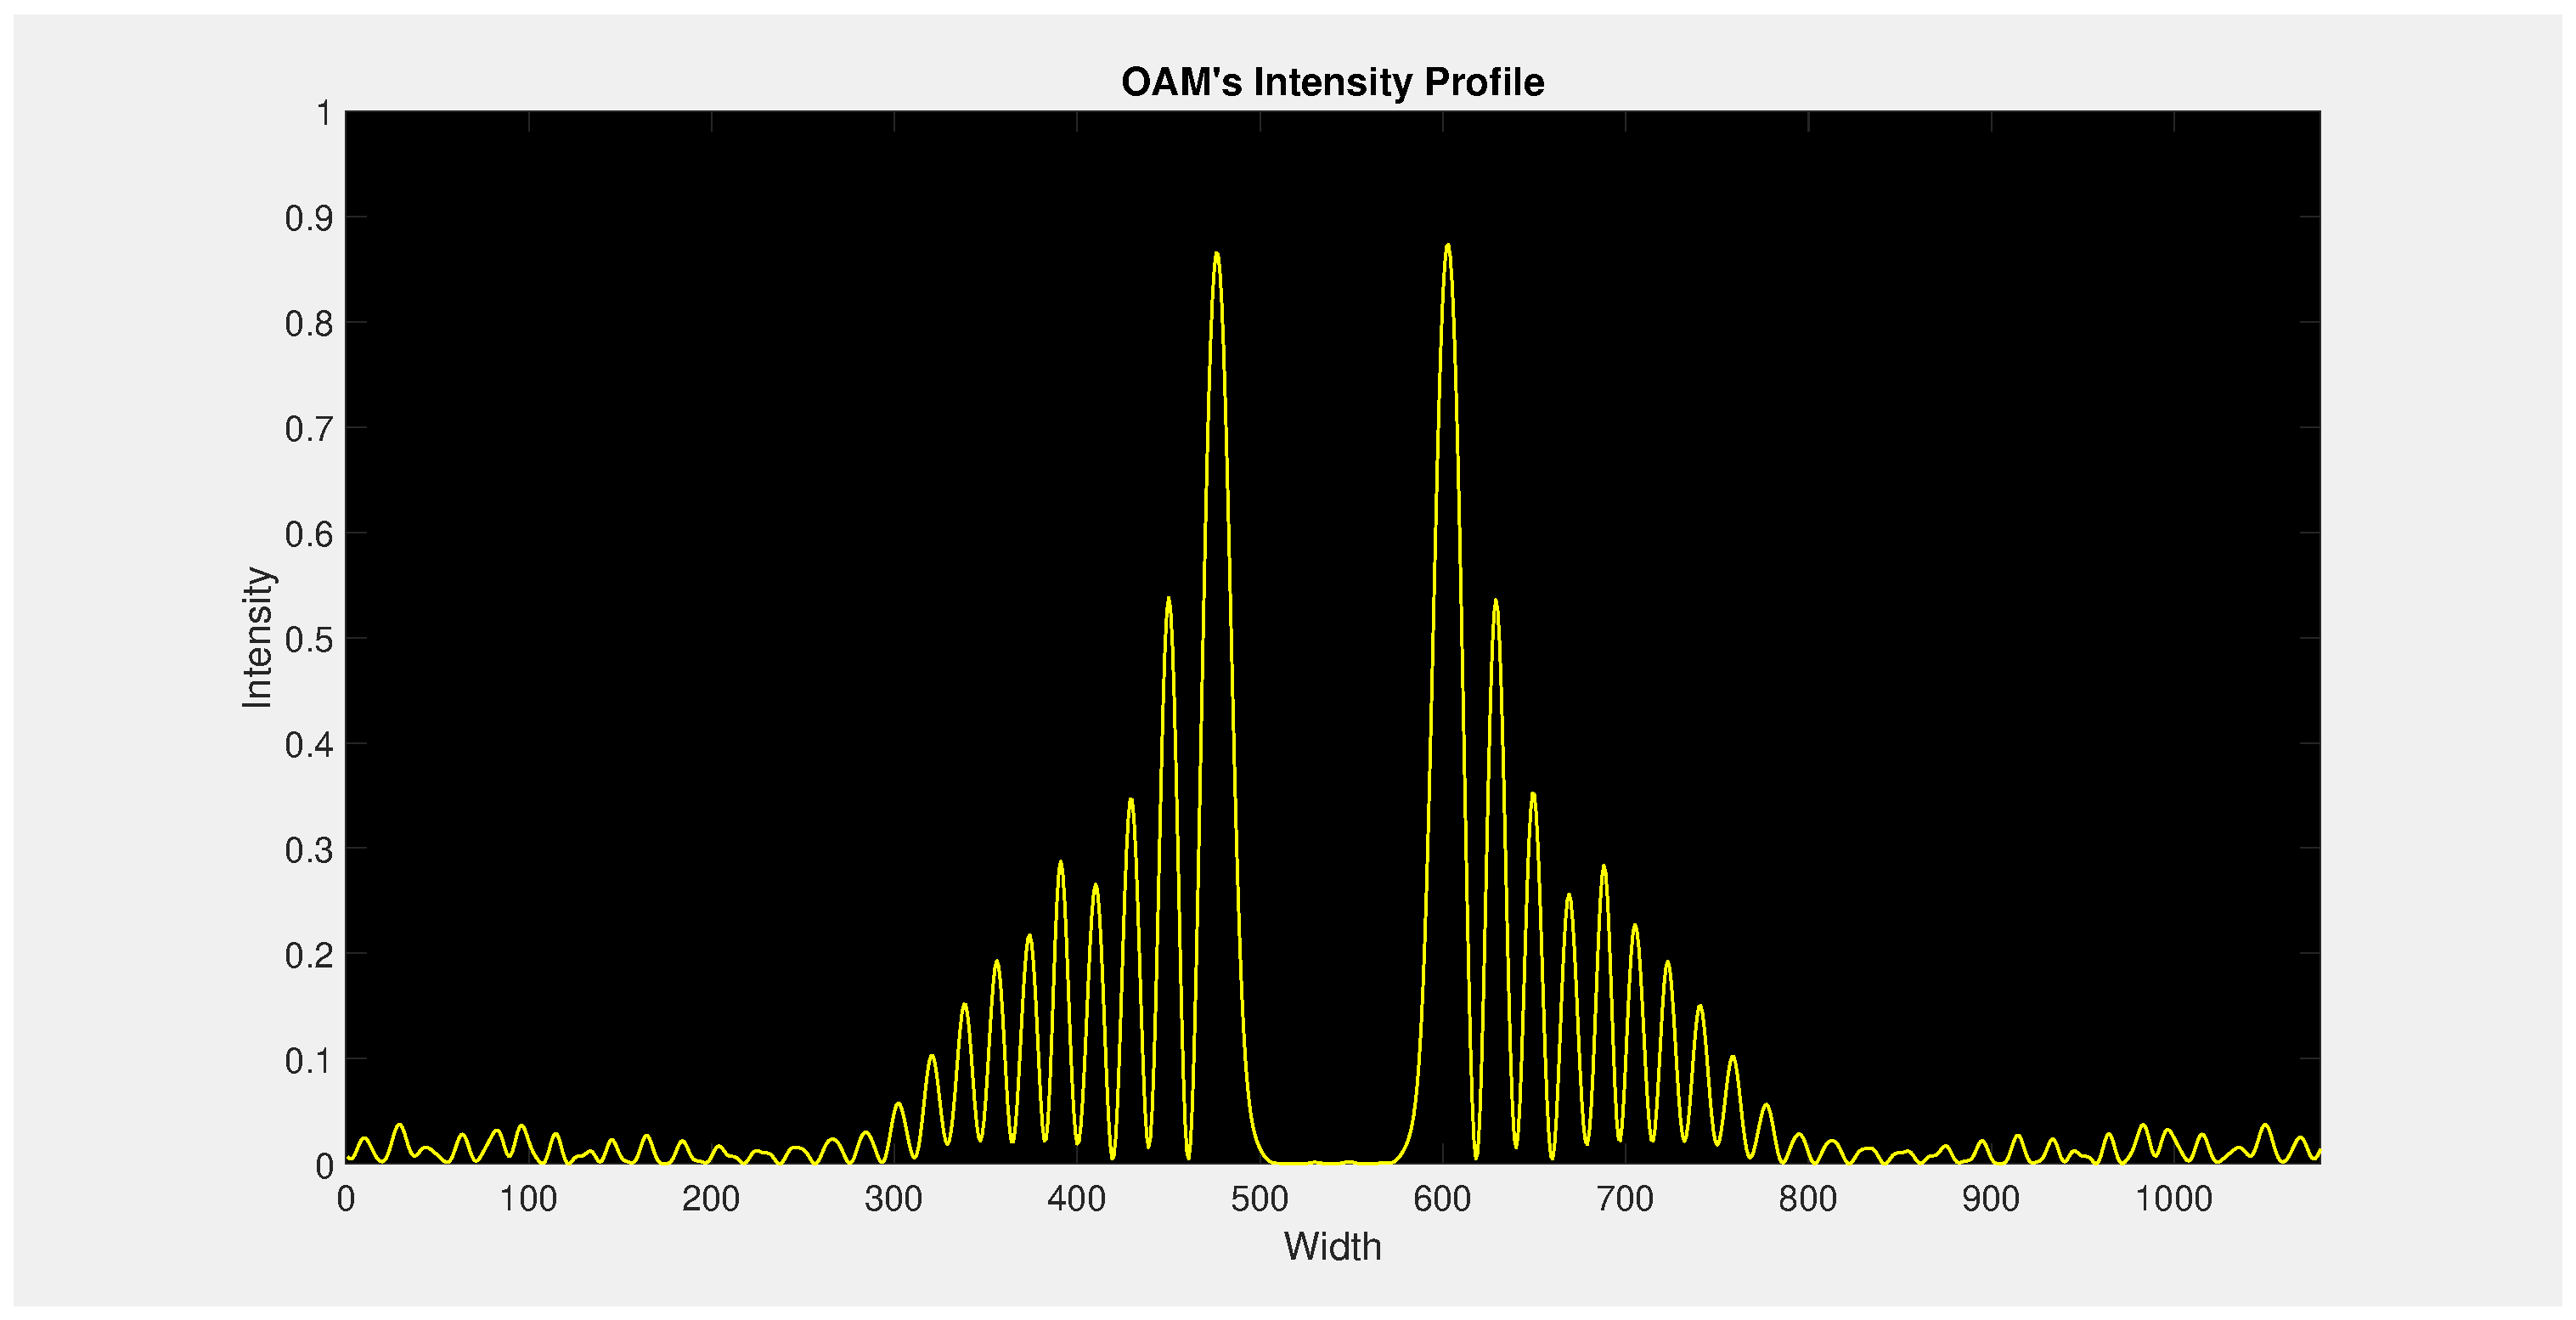
\includegraphics[width=\textwidth]{images/c02/OAM/Gaussian_Profile.eps}
        \caption{Intensity profile of the perfect vortex shown in figure (\ref{fig:Example_OAM}).}
        \label{fig:example_perfect_OAM_profile}
    \end{subfigure}
    \caption{Normalized intensity profiles. Notice how figure (\ref{fig:example_perfect_OAM_profile}) still follows the general shape of a Gaussian curve, as well as for each individual ring.}
    \label{fig:Example_Intesity_Profiles}
\end{figure}

\subsection{Making an OAM beam}
\label{c2:Making an OAM beam}

There are three commonly used methods to induce orbital angular momentum on a light beam. The first one is by combining Hermite-Gauss (HG) modes to generate Laguerre-Gaussian (LG) ones using a laser. Another one, is by using a spiral phase plate whose optical thickness varies linearly with the azimuthal angle. The final method consists of using a spatial light modulator (SLM) to project a \textit{phase mask}\footnote{Also referred to as \textit{hologram} or \textit{interference pattern plate}.} that sits in front of a typical laser beam and induces OAM on it. The phase mask is generated by the Laguerre-Gauss equation (\ref{Laguerre-Gauss Equation}) \cite{Anguita:08}.

\begin{figure}[htbp]
    \centering
    \begin{subfigure}[b]{0.3\textwidth}
        \centering
        \fbox{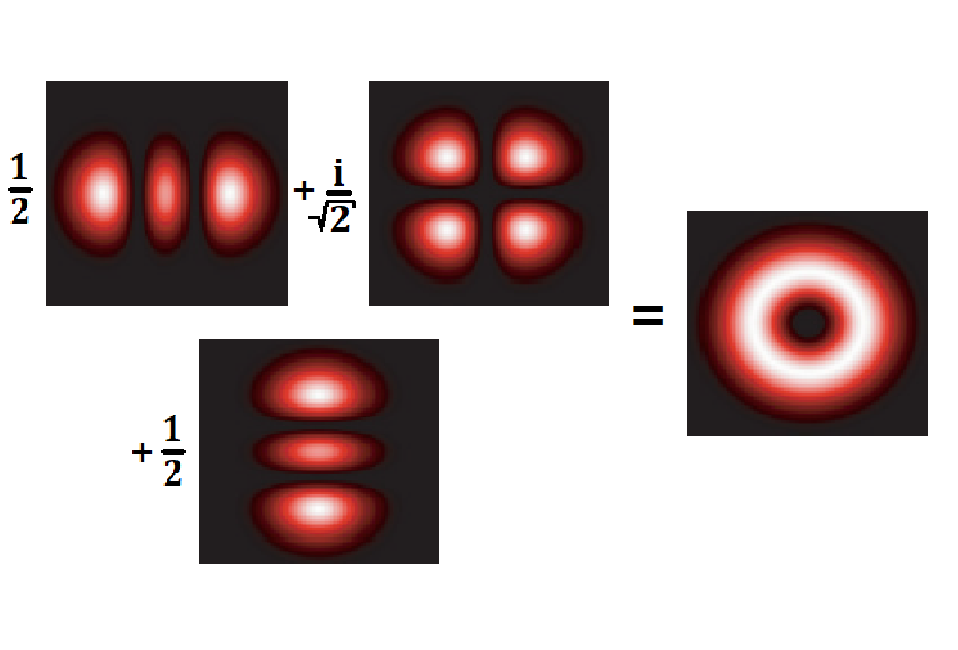
\includegraphics[width=\textwidth]{images/c02/OAM/HG_to_LG_resized.png}}
        \caption{First method: conversion from HG to LG modes \cite{Yao-Padgett:2011}.}
    \end{subfigure}
    \hfill
    \begin{subfigure}[b]{0.3\textwidth}
        \centering
        \fbox{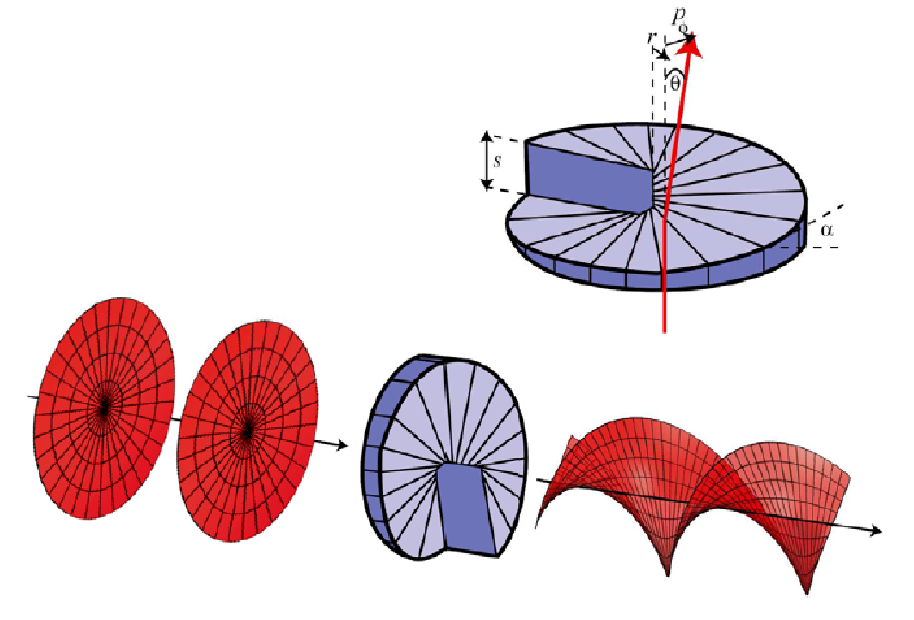
\includegraphics[width=\textwidth]{images/c02/OAM/OAM_Plate.PNG}}
        \caption{Second method: Using a spiral phase plate \cite{Yao-Padgett:2011}.}
    \end{subfigure}
    \hfill
    \begin{subfigure}[b]{0.3\textwidth}
        \centering
        \fbox{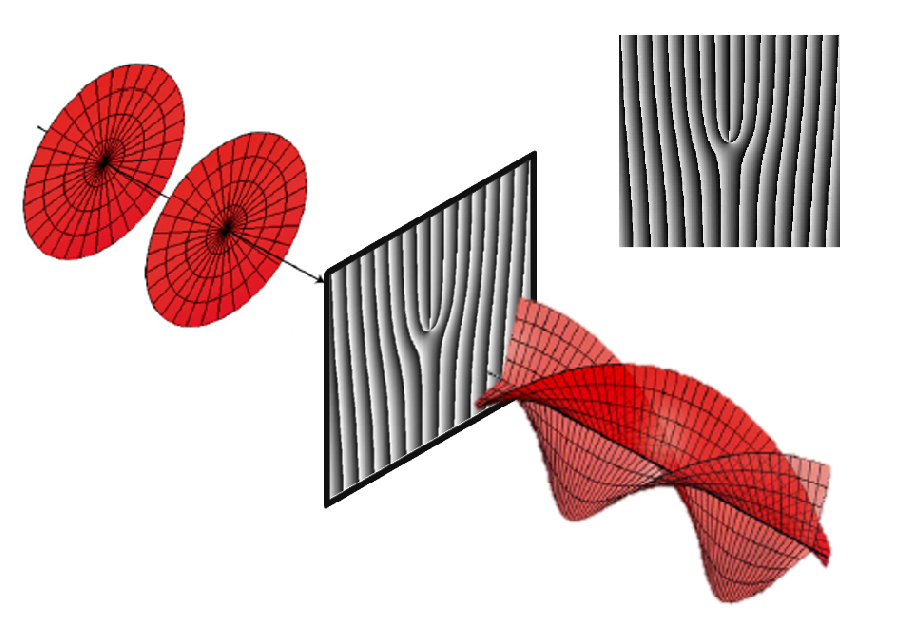
\includegraphics[width=\textwidth]{images/c02/OAM/Gaussian-Fork-OAM.png}}
        \caption{Third Method: Using a phase mask (Created by the author).}
    \end{subfigure}
    \caption{Illustration of all three methods to generate an optical vortex. Assuming each one is producing the same OAM's state, their outcomes should be the same vortex, in theory.}
    \label{fig:OAM_Generation_Methods}
\end{figure}

In the FICA\footnote{Spanish acronym for ``Facultad de Ingeniería y Ciencias Aplicadas''.} optics laboratory, the third method is preferred due to its simplicity and relatively cheap implementation, as the SLM's projection can change, allowing for flexibility in the variations of the experiments. Finally, because the SLM is controlled by a computer through a common DVI or HDMI cable, changing the setup is almost instantaneous without requiring physical modifications to the experiment table. Ultimately, to adhere as closely as possible to this condition, the work presented in this paper simulates this approach.

The Laguerre-Gauss equation that can generate different phase masks is \cite{Yao-Padgett:2011}:

\begin{eqnarray}
    LG_{\ell, p} = \sqrt{\frac{2p!}{\pi (p + |\ell|)!}}\frac{1}{w(z)}\left[ \frac{r\sqrt{2}}{w(z)} \right]^{|\ell|}exp\left[ \frac{-r^2}{w^2(z)} \right] L_p^{|\ell|} \left( \frac{2r^2}{w^2(z)} \right) exp[i\ell\phi]\nonumber\\exp\left[ \frac{ik_0r^2z}{2(z^2+z^2_R)} \right] exp \left[ -i(2p+|\ell|+1)\tan^{-1}{\left( \frac{z}{z_R} \right)} \right]
    \label{Laguerre-Gauss Equation}
\end{eqnarray}

Where the Gaussian's radius is given by the expression $w(z) = w(0)[(z^2+z^2_R)/z^2_R]^{1/2}$, $z$ is the beam's propagation distance, $w(0)$ is the beam's radius for $z=0$ (or beam ``waist''; see figure (\ref{fig:Gaussian_Beam_Waist})), $z_R$ is Rayleigh's range and $(2p+|\ell|+1)\tan^{-1}{(z/z_R)})$ is the Gouy phase\footnote{Defined as the phase changes that the beam experiments near its focal distance.}. The term $L_p^{|\ell|}(x)$ is a polynomial obtained from the Laguerre polynomials, described by the following expression:

\begin{equation}
    L_p^{|\ell|}(x) = (-1)^{|\ell|}\frac{d^{|\ell|}}{dx^{|\ell|}}L_{p+|\ell|}(x)
\end{equation}

Notice that Rayleigh's range $z_R$ is given by equation:

\begin{equation}
    z_R = \frac{\pi w_0^2n}{\lambda}
\end{equation}

Where $\lambda$ is the wavelength and $n$ is the medium's refractive index.

\begin{figure}[htbp]
    \centering
    \fbox{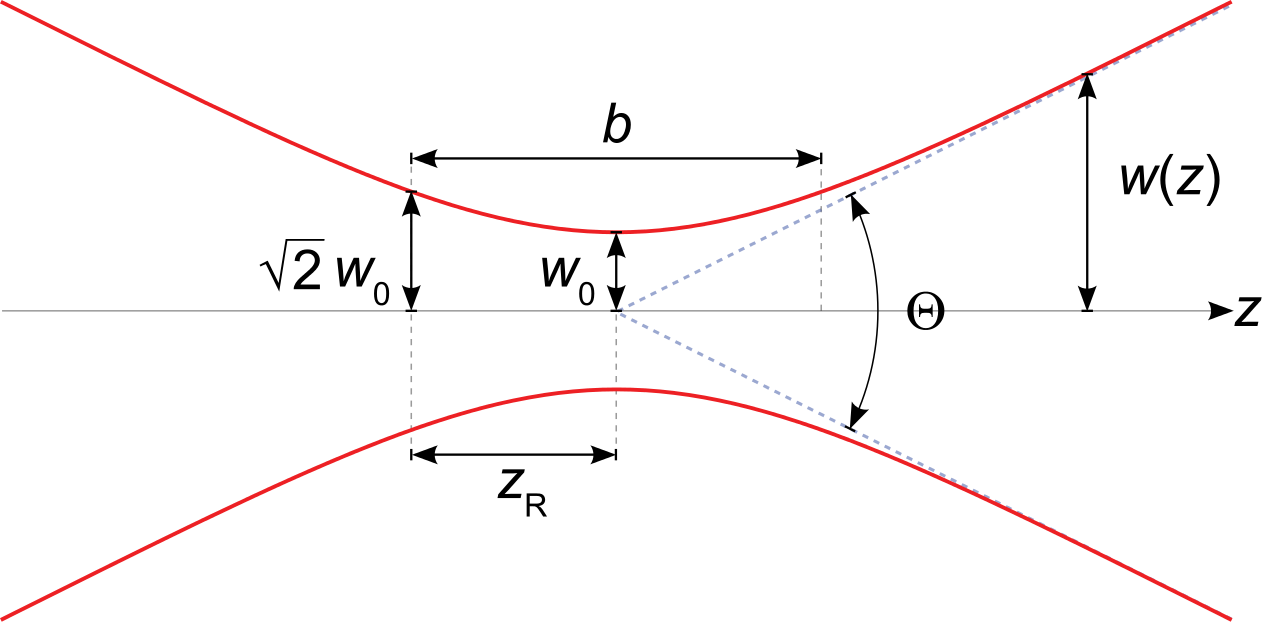
\includegraphics[width=8.5cm]{images/c02/OAM/GaussianBeamWaist.png}}
    \caption{Illustration of the Gaussian beam's waist \cite{GaussianBeamParameters}.}
    \label{fig:Gaussian_Beam_Waist}
\end{figure}

As it can be seen, the two input arguments of equation (\ref{Laguerre-Gauss Equation}) are $\ell$ and $p$, the latter representing the number of rings of the vortex. Examples of vortices with different values for these parameters are shown in figure (\ref{fig:OAMs_given_L_and_P}).

\begin{figure}[htbp]
    \centering
    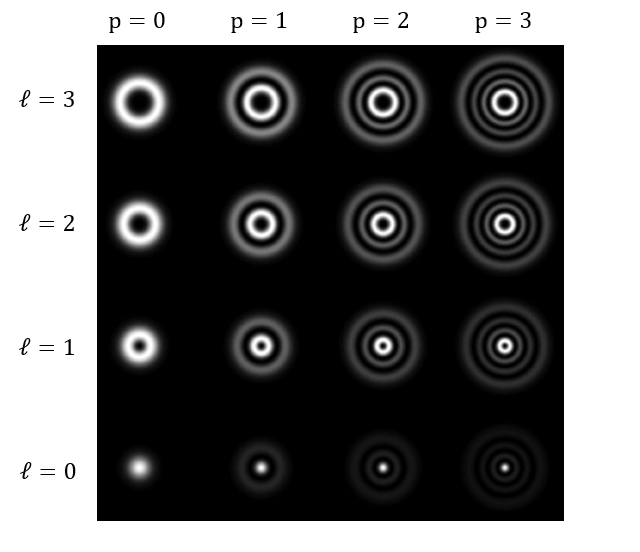
\includegraphics[width=9cm]{images/c02/OAM/OAM_given_L_and_P.png}
    \caption{Resulting optical vortices for different $\ell$ and $p$ values for equation (\ref{Laguerre-Gauss Equation}) \cite{OAM_states_Carbone:2013}.}
    \label{fig:OAMs_given_L_and_P}
\end{figure}

\newpage
\section{Near-Field and Far-Field Propagation Models}
\label{c2:Near and Far Field Propagation}

In order to simulate the propagation of an OAM beam, it is necessary to define the near-field and far-field diffraction models mathematically. They are used to resemble, as accurately as possible, the diffraction pattern generated by light passing through an aperture, assuming that the light source is coherent, which means that it emanates monochromatic wavefronts like that from a laser. 

The reason to distinguish between both near and far field scenarios, come from observing the changes that the outcome's intensity pattern experiences as the surface onto the which is projected is placed further away from the slit. A visual representation of this phenomenon is shown in figure (\ref{fig:Diffraction-Distinction}).

\begin{figure}[htbp]
    \centering
    \fbox{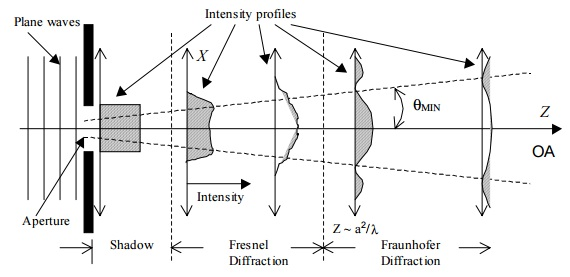
\includegraphics[width=10cm]{images/c02/Propagation/Fresnel-Fraunhoffer_Diffraction.jpg}}
    \caption{Illustration of varying intensity profiles as the projection is placed further from the slit \cite{Near-Far_Field_Diff}.}
    \label{fig:Diffraction-Distinction}
\end{figure}

There is a critical distance that serves to determine whether near field diffraction or far field one are to be used in a certain scenario. This distance is given by equation (\ref{near-far-field}) and it relates the beam's size and wavelength.

\begin{equation}
    d = \frac{2D^2}{\lambda}
    \label{near-far-field}
\end{equation}

Here, $d$ is the critical distance and $D$ is the beam's radius. Although there is not a more accurate definition, it is accepted that near field and far field are given by their relation with the critical distance, as follows.

\begin{eqnarray}
    z &>& d \implies \textrm{near field}\\
    z &>>& d \implies \textrm{far field}
\end{eqnarray}

In this fashion, the Fresnel diffraction or integral is defined as the contribution of each point $U_s$ from the plane at the beginning of the propagation, which is for $z = 0$ and defined by axes $x'$ and $y'$, onto the point $U_0$ within the propagated plane defined by axes $(x,y)$, as shown in figure (\ref{fig:Propagation_Diagram}).

\begin{figure}[htbp]
    \centering
    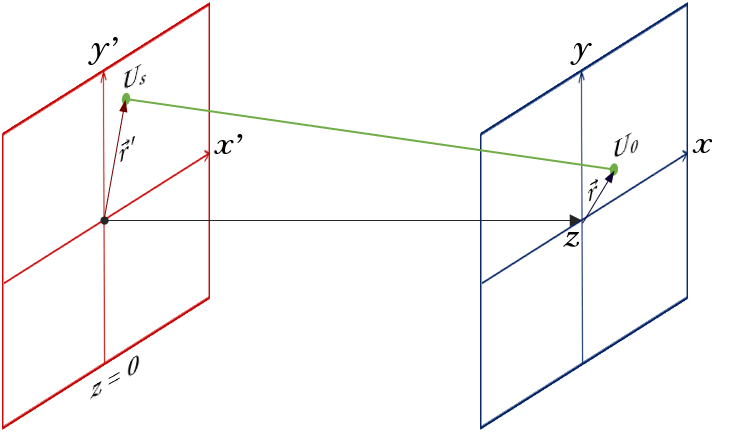
\includegraphics[width=9cm]{images/c02/Propagation/Propagation.png}
    \caption{Diagram of the propagation of a coherent wavefront from one plane onto another (Created by the author).}
    \label{fig:Propagation_Diagram}
\end{figure}

\begin{equation}
    U_0(x,y) = \frac{1}{i\lambda}\int_{-\infty}^{\infty}\int_{-\infty}^{\infty}\frac{U_s(x',y')e^{ik|\overrightarrow{r}-\overrightarrow{r}'|}}{|\overrightarrow{r}-\overrightarrow{r}'|}dx'dy'
    \label{Fresnel Integral}
\end{equation}

Here, the expression $|\overrightarrow{r}-\overrightarrow{r}'| = \sqrt{(x-x')^2+(y-y')^2+z^2}$ and $k = \frac{2\pi}{\lambda}$. We can simplify equation (\ref{Fresnel Integral}) by using the binomial expansion and paraxial approximation, respectively.

\begin{equation}
    \sqrt{(x-x')^2+(y-y')^2+z^2} = z\sqrt{1 + \left( \frac{x - x'}{z} \right)^2 + \left( \frac{y - y'}{z} \right)^2}
    \label{Binomial Expansion}
\end{equation}

\begin{equation}
    z\sqrt{1 + \left( \frac{x - x'}{z}^2 \right) + \left( \frac{y - y'}{z}^2 \right)} \approx z \left( 1 + \frac{1}{2} \left( \frac{x - x'}{z} \right)^2 + \frac{1}{2} \left( \frac{y - y'}{z} \right)^2 \right)
    \label{Paraxial Approximation}
\end{equation}

Considering that the propagation distance is significantly greater than the ``displacement'' that $U_0$ endures, with respect to $U_s$ it can be assumed that $z >> (x-x')$ and $z >> (y-y')$. This allows to nullify the terms in equation (\ref{Paraxial Approximation}) being divided by z, leaving the equation as $\approx z(1+0+0) = z$. Notwithstanding, is this approach in the denominator of equation (\ref{Fresnel Integral}), as it is scaled by $k$, which can enlarge errors not considered by the approximation and negatively alter the outcome. Taking this into consideration, the near field approximation is left obtained.

\begin{equation}
    U_0(x,y) = \frac{1}{i\lambda z}\int_{-\infty}^{\infty}\int_{-\infty}^{\infty}U_s(x',y')e^{ikz \left( 1 + \frac{1}{2} \left( \frac{x - x'}{z} \right)^2 + \frac{1}{2} \left( \frac{y - y'}{z} \right)^2 \right)}dx'dy'
\end{equation}

Finally, by moving the $x'$-and-$y'$-independent terms out of the integral, we are left with the simplified near field approximation.

\begin{equation}
    U_0(x,y) = \frac{e^{ikz}}{i\lambda z}e^{\frac{i\pi}{\lambda z}(x^2+y^2)}\int_{-\infty}^{\infty}\int_{-\infty}^{\infty}U_s(x',y')e^{\frac{i\pi}{\lambda z}(x'^2+y'^2)}e^{-i\frac{2\pi}{\lambda z} (xx'+yy')}dx'dy'
    \label{Near Field Approximation}
\end{equation}

On the other hand, the far field approximation assumes instead that the propagation distance is significantly greater than the the projection $U_0$ itself, or mathematically, $z >> x'^2$ and $z > y'^2$. Hence, the term $e^{\frac{i\pi}{\lambda z}(x'^2+y'^2)} \rightarrow 1$ because:

\begin{equation}
    \frac{x'^2}{z} \rightarrow 0, \frac{y'^2}{z} \rightarrow 0
\end{equation}

Therefrom, Fraunhoffer's approximation is obtained.

\begin{equation}
    U_0(x,y) = \frac{e^{ikz}}{i\lambda z}e^{\frac{i\pi}{\lambda z}(x^2+y^2)}\int_{-\infty}^{\infty}\int_{-\infty}^{\infty}U_s(x',y')e^{-i\frac{2\pi}{\lambda z} (xx'+yy')}dx'dy'
    \label{Far Field Approximation}
\end{equation}


It is also possible to rewrite this equation by using the Fourier transform, which is specially useful for MATLAB. Notice how the double integral resembles the 2D Fourier transform definition. By defining the variables $u = \frac{x}{\lambda z}$ and $v = \frac{y}{\lambda z}$, then this double integral can designate the Fourier Transform of some function $f_s(x',y')$

\begin{equation}
    U_0(x,y) = \frac{e^{i\frac{2\pi}{\lambda}}z}{i\lambda z}e^{i\pi \lambda z(x^2+y^2)}F_s(\frac{x}{\lambda z},\frac{y}{\lambda z})
\end{equation}
    % Objetivos

\chapter{Methodology} \label{Procedure}
\label{c3} % la etiqueta para referencias

\section{Context}
\label{c3:Methodology:Context}
% Maybe the following portion is more of a motivation rather than procedure.
The simulation is based on the optical setup shown in figure (\ref{fig:Simulated_Experiment}), which reproduces the existing setup in the FICA UANDES optics laboratory. It shares the core structure with other optical experiments that study, yet are not limited to, atmospheric turbulence, crosstalk and simple data transmission (Tx) and reception (Rx) analysis. However, the feature that is of most interesting for this case, is the telescope in the Rx side.

\begin{figure}[htbp]
    \centering
    \fbox{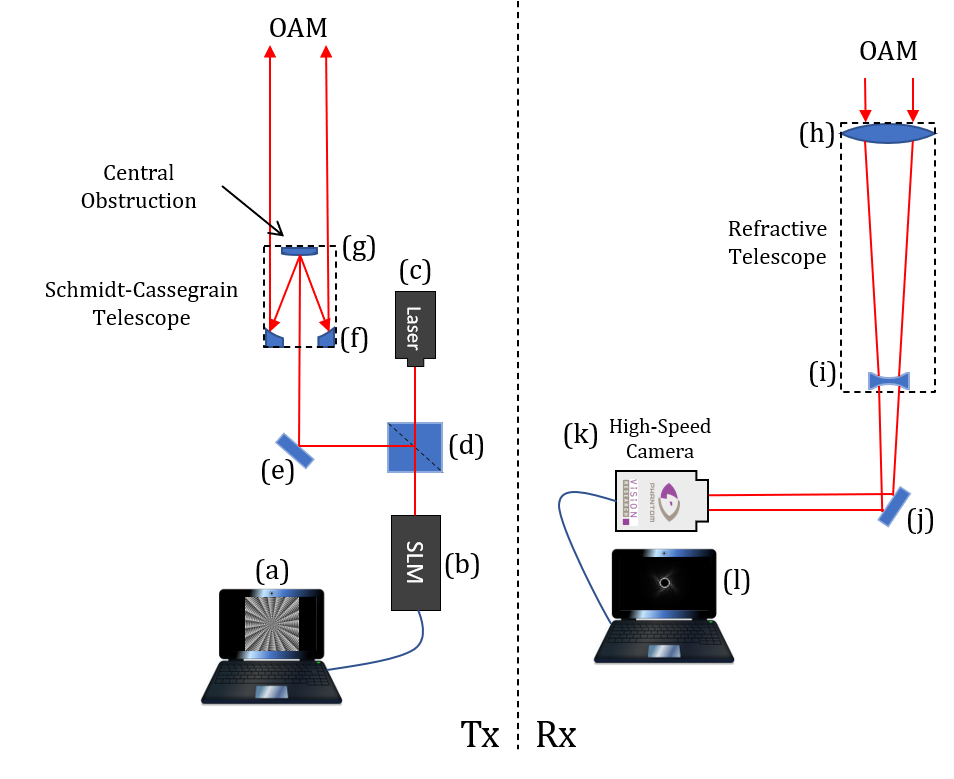
\includegraphics[width=7cm]{images/c03/Simulated_Experiment.png}}
    \caption{Diagram showing the simulated experiment.}
    \label{fig:Simulated_Experiment}
\end{figure}

\newpage
There is a myriad of telescopes, among the which the Schmidt-Cassegrain particularly stands out. It is one of the most used ones because it allows wide apertures devices to be built within a short cylinder (compared with its focal-length-equivalent refractor). The disadvantage that the Schmidt-Cassegrain encompasses, is its central obstruction, that serves as the resting location for the mirror that reflects and focuses incoming light towards the eyepiece ((i) in figure (\ref{fig:Simulated_Experiment})). For distant targets, this obstruction is inconsequential due to the parallax effect; nevertheless, for shorter distances, such as the ones that might be used in a laboratory, it becomes an obstacle for a vortex, as it can block its central singularity.

\begin{figure}[htbp]
    \centering
    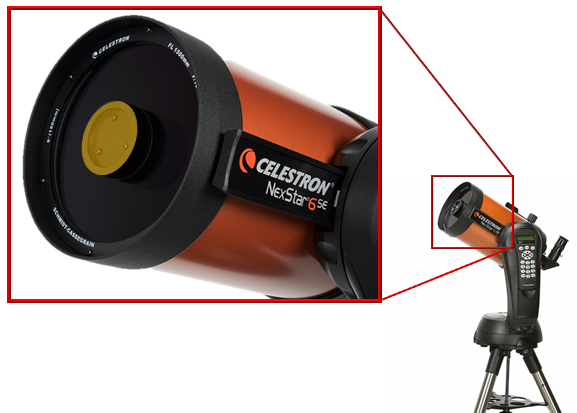
\includegraphics[width=7cm]{images/c03/Cassegrain-Obstruction.png}
    \caption{Schmidt-Cassegrain telescope like the one available in the FICA laboratory. The obstruction is colored in light yellow \cite{Schmidt-Cassegrain_Pics}.}
    \label{fig:Schmidt-Cassegrain-Obstruction}
\end{figure}

The simulation takes into consideration every aspect of this experiment: creation and propagation of the phase mask, central obstruction placement and intensity and topological charge analysis at the receiving end.

Because the obstruction in figure (\ref{fig:Simulated_Experiment}) is in the receiver system (although it could be relocated if the setup is modified) the concept of staged propagation is introduced. Staged propagation is intended to model a single circular-shaped central obstruction at any location within the propagation path. This concept may also model a regular, unobstructed propagation. Briefly explained, it simulates a phase mask to be propagated through a total distance $z_f$ measured in [mm] from the beginning (Tx), that encounters an obstruction located at $z_i$, also in [mm]. The obstruction size can vary, including a null size to model unobstructed propagations.

\section{Procedure}
\label{c3:Procedure}

The simulation is made possible thanks to ten MATLAB modules: nine functions and one main script, the latter called \textit{Obs\_Analysis\_Exe.m}. Of the nine functions, eight provide distinct aspects of the simulation, such as creating a specific image or describing a mathematical function along with their variables. The remaining function is the main one, called \textit{Obstruction\_Analysis.m}, which is the actual simulation of the setup shown in figure (\ref{fig:Simulated_Experiment}), and it makes use of the other eight functions in chronological order. The main script recalls the main function to obtain results with varying parameters to test diverse scenarios.

Do consider that the purpose of the following description is to present an overview of the simulation as a whole process. For a more detailed explanation on each function and script, their arguments, code revision and documentation, please refer to appendix \ref{MATLAB_Scripts}.

First of all, a phase mask is generated. The phase mask can be that of a regular vortex, generated by the function \textit{OAMgridFullHD\_GS.m}, or a perfect vortex, generated by the function \textit{OPE\_Mask.m}. In the main function, they are represented by argument \textit{type} which can take the values 0 or 1, respectively. Both types need a topological charge specified, represented by the argument \textit{state}, to generate the non-propagated mask at said state.

Then, the staged propagation takes place. As it was discussed in section \ref{c3:Methodology:Context}, the term of staged propagation is introduced in this paper. This method is better illustrated in the flow chart shown in figure (\ref{fig:staged_propagation_flow_chart}).

\begin{figure}[htbp]
    \centering
    \fbox{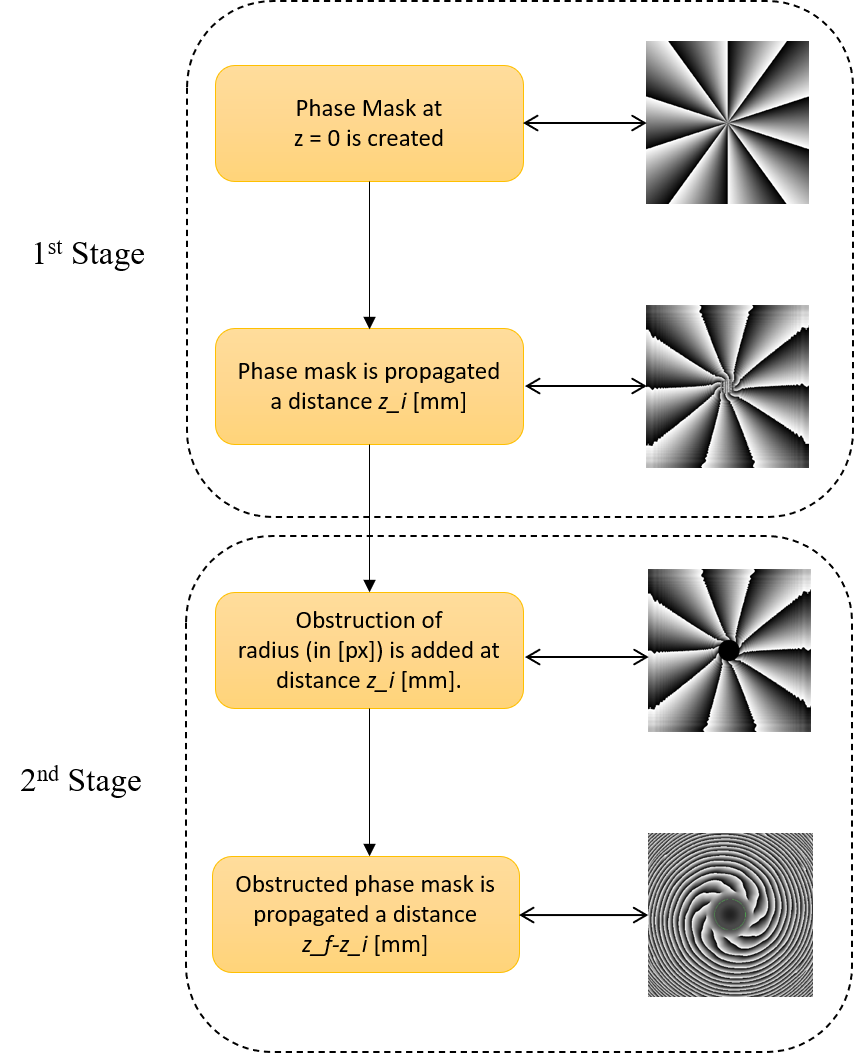
\includegraphics[width=7.5cm]{images/c03/Staged_Propagation_Flux_Chart.png}}
    \caption{Staged propagation flow chart along with per-stage visualizations of the mask along the path.}
    \label{fig:staged_propagation_flow_chart}
\end{figure}

Staged propagation receives as arguments the distances \textit{z\_i} and $z_f$, which are given in [mm], and the obstruction size, which is measured in pixels (px). If a direct propagation is desired, $z_i$ should be set to 0. If an unobstructed propagation is desired, the obstruction size, represented by the variable \textit{obstruction\_radius}, should be set to 0; in this case, it is recommended to do a direct propagation.

Once the propagation is simulated, the topological charge is estimated using the function \textit{Circ\_Profile.m}, that takes an intensity profile at the pixels of a circumference with a given radius, in [px]. This circular profile is taken on the propagated mask. By counting the number of peaks that the profile has, one can estimate the topological charge. The number of peaks are the number of ``creases'' that the image has, which should be the same number as the topological charge. Theses creases look like a line, which on one side are a very light gray or white, and on the other side are dark gray or black.

This whole process returns the data to produce two figures. The first one shows four images: the phase mask just before the obstruction, the propagated phase mask, the resulting vortex and its intensity profile. From now on, these images will be respectively referred by the names: unobstructed phase mask, propagated phase mast, vortex or OAM and intensity profile. The second figure shows the plot of the circular profile taken on the propagated phase mask. Examples of these can be seen in figures (\ref{fig:example_figure1}) and (\ref{fig:example_figure2}), respectively.

\begin{figure}[htbp]
    \centering
    \includegraphics[width=10cm]{images/c03/Example_Result.eps}
    \caption{Example figure of the first kind. The sub-figures seen are, clockwise from top-left, the phase mask at the obstruction's location, the propagated phase mask, the intensity profile and the vortex. The cyan circumference in the propagated phase mask shows where the circular profile was taken. Notice that in this example, obstruction radius is 0 [px], and therefore, there is no obstruction.}
    \label{fig:example_figure1}
\end{figure}

\begin{figure}[htbp]
    \centering
    \includegraphics[width=10cm]{images/c03/TC_example.eps}
    \caption{Example figure of the second kind. Notice that this plot is from a circular profile, meaning that the far right side of the graph directly continues on the far left side.}
    \label{fig:example_figure2}
\end{figure}

\newpage
All of the main function's arguments are listed below. Once again, if a more in-depth explanation is required, please refer to appendix \ref{MATLAB_Scripts}.

\begin{enumerate}
    \item \textit{img\_size}: Size of the image in [px]. All images generated are 1:1, i.e, a square of side \textit{img\_size}.
    \item \textit{state} ($\ell$): Topological charge. An integer is expected.
    \item \textit{z\_i}: First stage propagation distance in [mm]; denoted as $z_i$ in this work.
    \item \textit{z\_f}: Total propagation distance in [mm]. Second stage propagation distance is given by $z_f - z_i$ [mm]. Denoted as $z_f$ in this work.
    \item \textit{profile\_radius}: Profile radius in [px]. Any value can be used, as long as it is lower than half the image size.
    \item \textit{type}: Type of vortex. $type = 0$ represents regular vortices and $type = 1$ perfect vortices. Any other value will produce an error.
    \item \textit{obstruction\_radius}: Obstruction radius in [px]. Values higher than 100 are not recommended.
    \item \textit{sigma} ($\sigma$): Standard deviation of the 2D Gaussian that generates regular vortices. It is used to control the size of the Gaussian, where larger values return larger beams.
    \item \textit{Rpx}: Aperture size in [px]. The main function converts this measure to [mm] internally. The expected value is 764 [px]; however, under a slightly different scenario (to be presented later on) it can be set at 500 [px].
    \item \textit{N}: Number of Bessel's zeroes and number of rings. Values expected here are integers between 30 and 60.
\end{enumerate}

Arguments (i) and (j) were inherited from Bravo's undergraduate thesis \cite{Thesis_Herbert:2020}. He established the acceptable values' range for aperture and number of rings, in order to create a perfect vortex, by following the vortex's definition: a beam with a main ring that concentrates most of the beam's light intensity and a black center region, completely absent of light. He confirmed this by taking multiple intensity profiles on the vortices produced by these values.

Other arguments are implicit within some of the functions. For instance, the image size was set to 1080x1080 [px] because the UANDES optics' laboratory SLMs (Spatial Light Modulator) has a native resolution of 1920x1080 [px] (width and height, respectively) and 1080 [px] is the smallest side. Additionally, both functions, \textit{Fresnel.m} and \textit{OAMgridFullHD\_GS.m}, consider that the wavelength of the laser used is the same as the ones available in the laboratory, $660 \times 10^{-6}$ [mm], or equivalently 660 [nm]. In a similar fashion, the circular profile's radius is fixed to a value of 200 [px]; although this value could vary depending on the size of the obstruction or some other reference, after several iterations it was concluded that a large-enough fixed value delivered more accurate estimates. The other arguments were created by the author for this work.

\section{Main Script Usage}

The objective of this section is to instruct the reader on how to use the main script and how to input the arguments to obtain results of different nature.

First, the variables of the program are prompted to the user by the MATLAB script \textit{Obs\_Analysis\_Exe.m}. It is useful to distinguish fundamental variables from scenario variables. Fundamental variables are understood to be variables that affect the vortices themselves, and do not play a role in the obstruction nor propagation. On the other hand, scenario variables are the opposite.

For regular vortices, the fundamental variable is $\sigma$, and for perfect vortices, these are $N$ and $Rpx$. For most cases, these variables are best left unchanged, as a $\sigma = 100$ generates regular vortices correctly for practically all distances, from near-field to infinity. On the other hand, Herbert's work on perfect vortices concluded that the best vortices are produced by setting $N = \{40,60\}$ and $Rpx = 764$ [px] (roughly equivalent to 6.11 [mm]). During the course of this work, it was discovered that the range of $N$ can be expanded to $\{30,60\}$ without altering the outcome negatively. It was also discovered that the $Rpx$ can also be equal to $500$ (roughly equivalent to 4 [mm]); however, in order to procure a good vortex, the total propagation distance should be increased by approximately 30\% over its value at the time of using $Rpx = 764$ [px]. But that as it may, these discoveries did not seem to provide more interesting data than what was already available. In consequence and for the purpose of this work's main results, the fundamental variables were fixed at values within the margins previously described.

Moving on to scenario variables, the program gives the user the faculty to obtain results using different combinations of values by iterating to contemplate all possible combinations of them. For instance, say that the user wants to obtain results for unobstructed vortices, regular and perfect, of $\ell = 10$, but for different propagation distances, say 500 [mm] and 1000 [mm]. They should simply separate the desired evaluation values with a space, and the program iterates over all given combinations. In that event, the results' folder will contain eight images: four for perfect vortices and other four for regular vortices. Furthermore, each propagation produces two figures: one for the phase masks, vortex and its intensity profile, and a second one for the topological charge measurement, giving a grand total of 16 images (two per vortex). Therefore, it would really be considering two scenarios for each type of vortex, just as it was expected by only varying the total propagation distance (``Stage 2 Distances'' in the window). The previous case can be extended to all sorts of combinations and scenarios considering these variables.

In general, the number of cases is given by the multiplication between the total number of types of vortex, stages 1 and 2 distances and obstruction radii. This produces twice as much images, because each scenario produces two figures.

\begin{figure}[htbp]
    \centering
    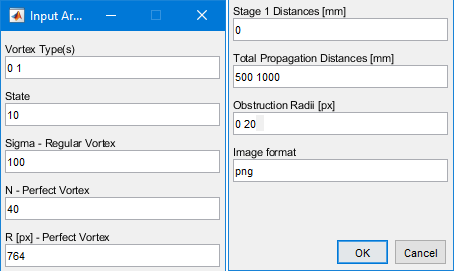
\includegraphics[scale=0.85]{images/c03/Input_Window_MATLAB_divided_v2.PNG}
    \caption{\textit{Obs\_Analysis\_Exe.m} prompt window filled out to obtain the results described above. The window was cut in half for better visualization in this document.}
    \label{fig:input_window}
\end{figure}

\newpage
Running the program with the parameters shown in figure (\ref{fig:input_window}), will result in the creation of the following folder and sub-folders, when the image format type is \textit{png}\footnote{Because Windows does not allow to preview \textit{eps} files by default, it is not necessary to classify them to preview them, as the names are self-explanatory. However, Windows does allows \textit{png} files to be previewed; in consequence, the program is designed to classify them to allow the user to scroll through the images continuously without interruptions such as showing a different type of vortex or figure.}. The images inside these folders are of the same type as figures (\ref{fig:example_figure1}) and (\ref{fig:example_figure2}).

\begin{figure}[htbp]
    \centering
    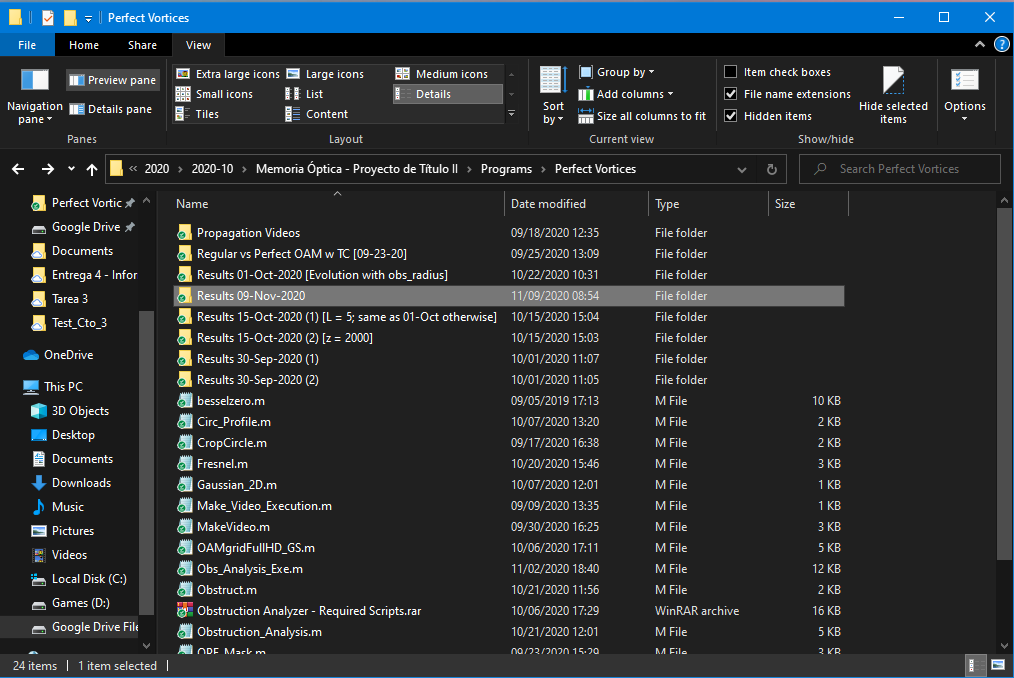
\includegraphics[width=11cm]{images/c03/General_Folder.PNG}
    \caption{Created folder (highlighted in gray) with the resulting images. Notice that its named (automatically) after the date it was created. If a folder with the same name already exists, the suffix (i) is placed, where i is the smallest available natural number.}
    \label{fig:general_folder}
\end{figure}

\begin{figure}[htbp]
    \centering
    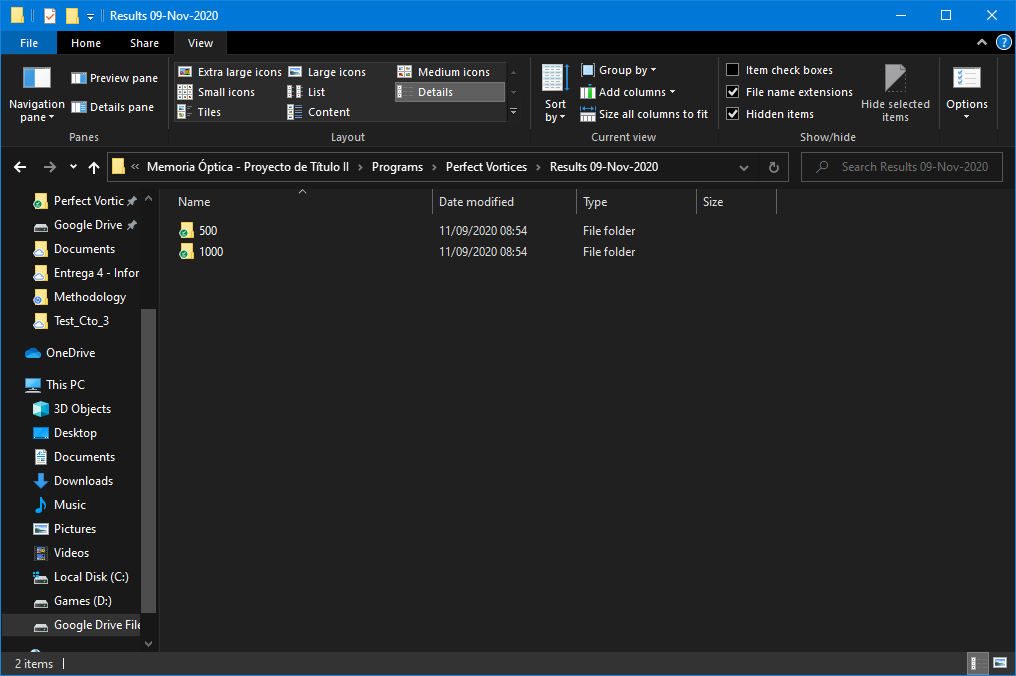
\includegraphics[width=11cm]{images/c03/Folder.PNG}
    \caption{Inside the created folder, where the images are classified by their propagation distance.}
    \label{fig:folder}
\end{figure}

\begin{figure}[htbp]
    \centering
    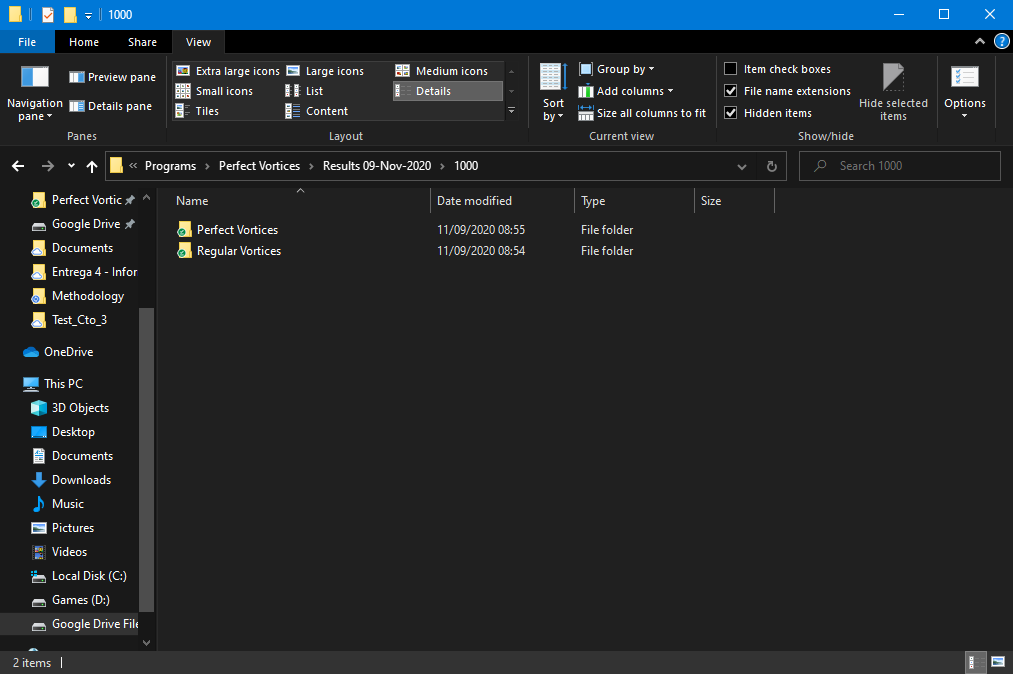
\includegraphics[width=11cm]{images/c03/Specific_folder.PNG}
    \caption{View inside one of the propagation distances' folder, specifically the z=1000 for this case. At this level, the sub-folders are classified by vortex type.}
    \label{fig:specific_folder}
\end{figure}

\begin{figure}[htbp]
    \centering
    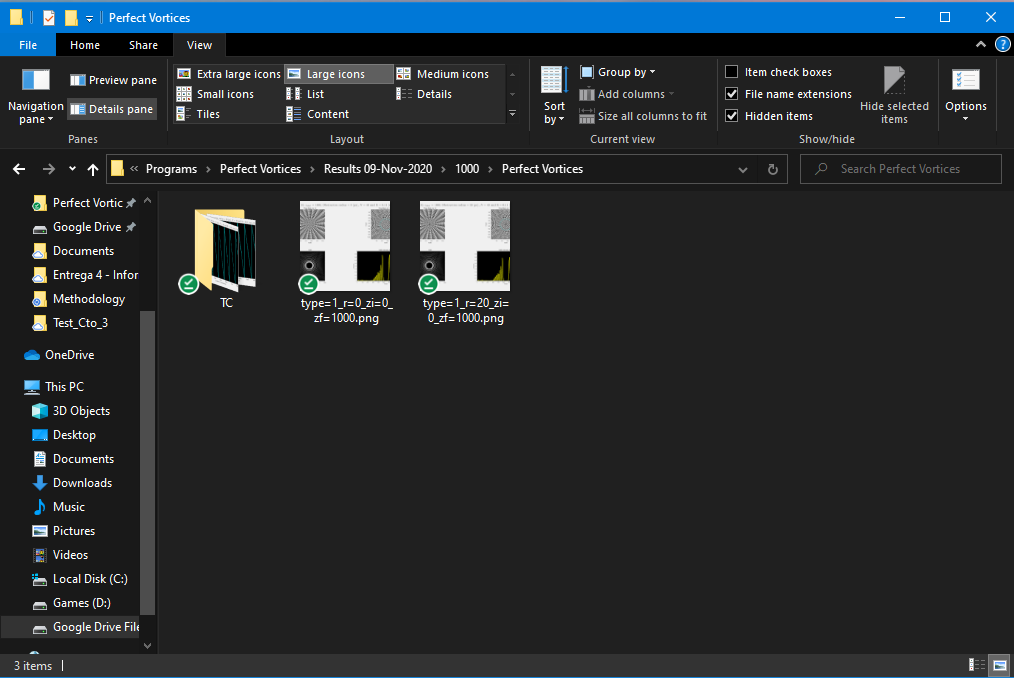
\includegraphics[width=11cm]{images/c03/Final_Folder.PNG}
    \caption{Inside one of the vortices type's folder, specifically the perfect vortices, the images are located. Their topological charges' plots are in a separate folder called ``TC''.}
    \label{fig:final_folder}
\end{figure}

\begin{figure}[htbp]
    \centering
    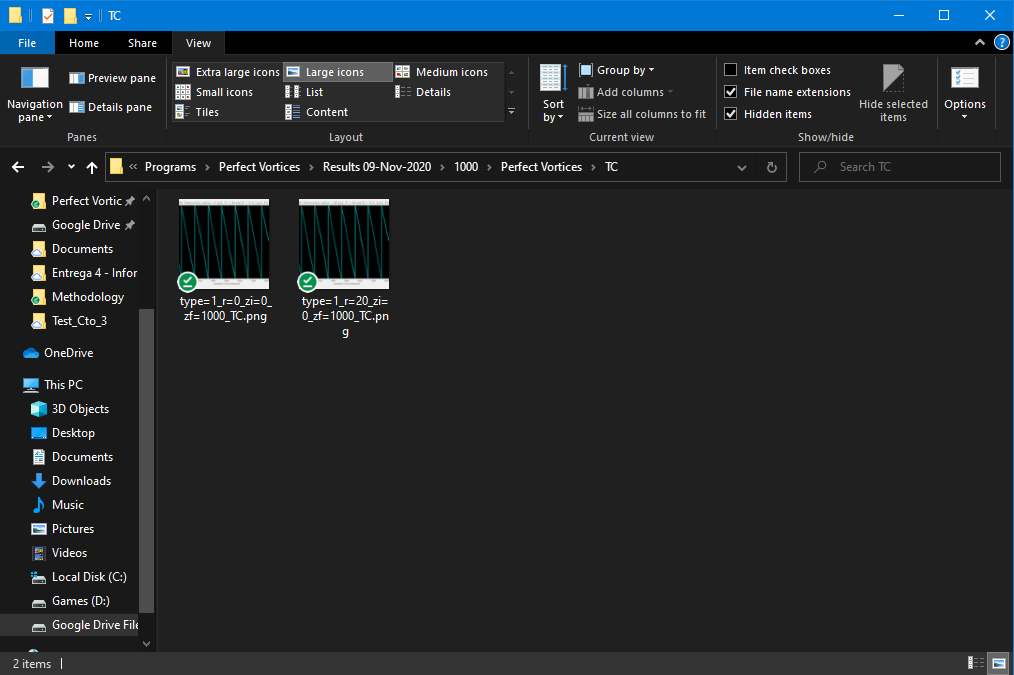
\includegraphics[width=11cm]{images/c03/Final_Folder_TC.PNG}
    \caption{View inside the TC folder.}
    \label{fig:final_folder_TC}
\end{figure}

\newpage
Notice that each image is named by its parameters \textit{type}, meaning the vortex's type; \textit{r}, meaning its obstruction radius; $z_i$ and $z_f$. The topological charge images are also named in this manner, with the addition of the suffix ``\_TC'' to distinguish them.

\begin{figure}[htbp]
    \centering
    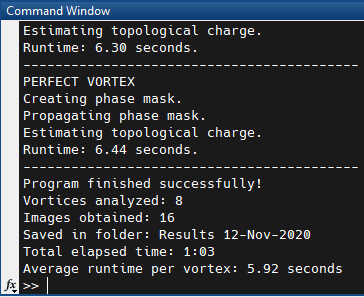
\includegraphics[width=9cm]{images/c03/Console_Output.PNG}
    \caption{Part of the console output obtained from executing the program \textit{Obs\_Analysis\_Exe.m} using the parameters shown in figure (\ref{fig:input_window}).}
    \label{fig:my_label}
\end{figure}

Finally, the console output displays two types of information blocks. Each block is separated by a dashed line. The first type shows the information of the latest single cycle, including vortex type, which stage of the program was executing at the moment (prints in real time) and the total runtime of that cycle. This is the most common block type and, naturally, it appears as many times as there are cycles. The second type is the last block, and is a summary of the complete execution, showing the folder's name where the images were saved (``Saved in folder'', in the above figure), total number of images and vortices, total elapsed time and a time average per cycle.

    % Metodología

\chapter{Results} \label{Results}
\label{c4} % la etiqueta para referencias

There are hundreds of possible combinations that can be analyzed by varying the arguments' value and iterations. The main course taken in this chapter is taking essential variations in propagation distance and vortex type and observe how they change as obstructions of larger sizes are imposed over them, and how they compare to the same vortex unobstructed. These results are consistent through changes in state, aperture and number of rings; these results can be further examined in appendix (\ref{Complementary_Results}).

%As it was said in the previous section, the fundamental arguments that generate the phase masks themselves, were not altered to produce the results presented in this section; however, some tests were made varying topological charge and fundamental arguments to test how they affected the outcome. It was decided not include these results here, but in appendix (\ref{Complementary_Results}), for they didn't produce interesting results, in the sense that they didn't provide information that was either new nor useful. On the other hand, variations in staged propagation, distances and obstructions' radii did yield some interesting insights.

As explained in section (\ref{c2:OAM}), the main structure of a vortex consists of a main ring that concentrates most of the beam's intensity, along with a pitch dark central region, consequence of the phase singularity that OAM induces on a beam.

When analyzing the following results, one should be mindful about the inaccuracies that simulations embrace when compared to real life scenarios. For instance, phase masks are not accurate representations, mainly for two reasons: (i) Propagation models introduce errors caused by digital approximations, specifically in the Fourier transforms, integrals and the limited resolution, and (ii) the amount of simultaneous variables that these must handle (refer to figure (\ref{fig:Propagation_Diagram})). In contrast, intensity figures (the OAMs) do represent reality very accurately, meaning that the simulations' results could be easily reproduced in an actual experimental setup.

A final note on how to read the images in this chapter: Most of the images presented here are in \textit{eps} format, meaning that they are vector images. The reader is encouraged to zoom into the images, to unveil more fine details, as no loss of quality will be perceived using a \textit{pdf} reader.

\section{Study of different obstruction radii sizes}
\label{c4: radii size variations}

In this section, $\sigma$, \textit{Rpx} and \textit{N} are fixed at their default values and shown in the title of each figure. Obstructions can deform and compromise the integral ``structure'' of an OAM beam, as described at the beginning of this chapter. Withal, as the obstructions enlarge, these deformations become more prominent, in both cases; however, regular vortices seem to deform more rapidly than perfect ones. 

The aforementioned observations can be examined in figures (\ref{fig:Vortices_r=0_z=1000}) and (\ref{fig:Vortices_r=30_z=1000}); keep in mind that images of perfect vortices (all sub-figures (b) below, bottom-left image titled ``OAM'') are zoomed-in to better visualize them. The first figure shows both regular ((a), left sub-figure) and perfect ((b), right sub-figure) vortices unobstructed (\textit{obstruction\_radius} = 0) and propagated directly through a total distance of 1000 [mm] (\textit{z\_i} = 0 and \textit{z\_f} = 1000). 

Because these vortices are unobstructed, they do not present deformations whatsoever. Their topological charge plot show in figure (\ref{fig:Vortices_r=0_z=1000_TC}) show them both at 10 prominent peaks, representing their topological charge, which is also 10. An examination on their normalized intensity profiles (bottom-right sub-figures, titled ``OAM's Intensity Profile'') confirms this. The two most prominent peaks, that represent the main ring, are practically maxed out, and they form a valley of null intensity, or darkness; this is true for both types.

\begin{figure}[htbp]
    \centering
    \begin{subfigure}[b]{0.45\textwidth}
        \centering
        \includegraphics[width=\textwidth]{images/c04/type=0_r=0_zi=0_zf=1000.eps}
        \caption{Regular vortex.}
    \end{subfigure}
    \hfill
    \begin{subfigure}[b]{0.45\textwidth}
        \centering
        \includegraphics[width=\textwidth]{images/c04/type=1_r=0_zi=0_zf=1000.eps}
        \caption{Perfect vortex.}
    \end{subfigure}
    \caption{Unobstructed vortices directly propagated through $z_f = 1000$ [mm].}
    \label{fig:Vortices_r=0_z=1000}
\end{figure}

\begin{figure}[htbp]
    \centering
    \begin{subfigure}[b]{0.45\textwidth}
        \centering
        \includegraphics[width=\textwidth]{images/c04/type=0_r=0_zi=0_zf=1000_TC.eps}
        \caption{Regular vortex.}
    \end{subfigure}
    \hfill
    \begin{subfigure}[b]{0.45\textwidth}
        \centering
        \includegraphics[width=\textwidth]{images/c04/type=1_r=0_zi=0_zf=1000_TC.eps}
        \caption{Perfect vortex.}
    \end{subfigure}
    \caption{Unobstructed vortices' topological charge.}
    \label{fig:Vortices_r=0_z=1000_TC}
\end{figure}

This is not the case for the obstructed vortices of figure (\ref{fig:Vortices_r=30_z=1000}), where an obstruction of radius 30 [px] was placed upon both type of vortices' phase masks ahead of their respective propagations. As a result, the propagated phase masks (top-right image of each subfigure) and OAMs were deformed. Nonetheless, by once again examining their intensity profiles, the deformations, and lack thereof, are unmistakable. 

In the case of the regular vortex, where its central dark region should be, as seen in the unobstructed scenario, a dim light is found, represented by a small hill in-between the two prominent peaks that are part of the main ring. Additionally, the main ring and its surrounding backlight experienced some sort of deformation, resembling the shape of a camera's shutter. Although the perfect vortex did suffer from loss of intensity in its main ring, slight deformations along its inner edge, and a scritcly non-dark valley, they are not as integral or critical as it was for the regular vortex. 

\begin{figure}[htbp]
    \centering
    \begin{subfigure}[b]{0.45\textwidth}
        \centering
        \includegraphics[width=\textwidth]{images/c04/type=0_r=30_zi=0_zf=1000.eps}
        \caption{Regular vortex.}
    \end{subfigure}
    \hfill
    \begin{subfigure}[b]{0.45\textwidth}
        \centering
        \includegraphics[width=\textwidth]{images/c04/type=1_r=30_zi=0_zf=1000.eps}
        \caption{Perfect vortex.}
    \end{subfigure}
    \caption{Vortices directly propagated through $z_f = 1000$ [mm] with a 30 [px] obstruction radius.}
    \label{fig:Vortices_r=30_z=1000}
\end{figure}

This deformations become more evident for both types as the obstruction size grows to 50 [px] of radius, as shown in figure (\ref{fig:Vortices_r=50_z=1000}). Here, the regular vortex already lost a core property: the region inside the main ring is now brighter than the main ring. As for the perfect one, the region inside the main ring now is covered by a very small, bumpy hill. Despite this, the main ring is still the most intense region and the outer rings have preserved their shapes.

\begin{figure}[htbp]
    \centering
    \begin{subfigure}[b]{0.45\textwidth}
        \centering
        \includegraphics[width=\textwidth]{images/c04/type=0_r=50_zi=0_zf=1000.eps}
        \caption{Regular vortex.}
    \end{subfigure}
    \hfill
    \begin{subfigure}[b]{0.45\textwidth}
        \centering
        \includegraphics[width=\textwidth]{images/c04/type=1_r=50_zi=0_zf=1000.eps}
        \caption{Perfect vortex.}
    \end{subfigure}
    \caption{Vortices directly propagated through $z_f = 1000$ [mm] with a 50 [px] obstruction radius.}
    \label{fig:Vortices_r=50_z=1000}
\end{figure}

\begin{figure}[htbp]
    \centering
    \begin{subfigure}[b]{0.45\textwidth}
        \centering
        \includegraphics[width=\textwidth]{images/c04/type=0_r=50_zi=0_zf=1000_TC.eps}
        \caption{Regular vortex.}
    \end{subfigure}
    \hfill
    \begin{subfigure}[b]{0.45\textwidth}
        \centering
        \includegraphics[width=\textwidth]{images/c04/type=1_r=50_zi=0_zf=1000_TC.eps}
        \caption{Perfect vortex.}
        \label{subfig:Perfect_r=50_z=1000}
    \end{subfigure}
    \caption{Topological charge of vortices propagated through $z_f = 1000$ [mm] with a 50 [px] obstruction radius.}
    \label{fig:Vortices_r=50_z=1000_TC}
\end{figure}

That being said, a quick examination to the topological charge of these obstructed vortices reveals that, apparently, their topological charge has not suffered significant changes.

Finally, with an obstruction of 100 [px] of radius (figure (\ref{fig:Vortices_r=100_z=1000})), the regular vortex essentially becomes a Gaussian beam surrounded by petal-like spotlights. Now the perfect one's central region is now uniformly lit; nonetheless, the main ring still is the most intense region. Do notice that the outer rings have now deformed as much as the central ring. Even though the main structure visually appears to be there, the intensity profile alerts that the center might be giving out a critical compromise.

\begin{figure}[htbp]
    \centering
    \begin{subfigure}[b]{0.45\textwidth}
        \centering
        \includegraphics[width=\textwidth]{images/c04/type=0_r=100_zi=0_zf=1000.eps}
        \caption{Regular vortex.}
    \end{subfigure}
    \hfill
    \begin{subfigure}[b]{0.45\textwidth}
        \centering
        \includegraphics[width=\textwidth]{images/c04/type=1_r=100_zi=0_zf=1000.eps}
        \caption{Perfect vortex.}
    \end{subfigure}
    \caption{Vortices directly propagated through $z_f = 1000$ [mm] with a 100 [px] obstruction radius.}
    \label{fig:Vortices_r=100_z=1000}
\end{figure}

\begin{figure}[htbp]
    \centering
    \begin{subfigure}[b]{0.45\textwidth}
        \centering
        \includegraphics[width=\textwidth]{images/c04/type=0_r=100_zi=0_zf=1000_TC.eps}
        \caption{Regular vortex.}
    \end{subfigure}
    \hfill
    \begin{subfigure}[b]{0.45\textwidth}
        \centering
        \includegraphics[width=\textwidth]{images/c04/type=1_r=100_zi=0_zf=1000_TC.eps}
        \caption{Perfect vortex.}
    \end{subfigure}
    \caption{Topological charge of vortices propagated through $z_f = 1000$ [mm] with a 100 [px] obstruction radius.}
    \label{fig:Vortices_r=100_z=1000_TC}
\end{figure}

On the side of the topological charge, once again, it does not show relevant changes. Although one might notice that the perfect vortex's plot has curvier ramps, it does not affect the number of peaks, which holds at 10, as it is expected. This helps us to conclude that, even though the obstruction size does significantly affect the shape and structure of the OAM in intensity, it does seem to reflect such drastic shifts in its phase, at least not enough to alter the topological charge.

In summary, this set of results show that regular vortices are more susceptible to deformation when coming across a central circular obstruction, in comparison to perfect vortices.

\section{Study of different propagation distances}
\label{c4:z_f variations}

Following the same logic line, this section studies the outcomes of changing the final propagation distance, mainly. Regardless, a similar evolution for $z_f = \infty$ will be presented as well. 

At 1500 [mm] and an obstruction of 50 [px] of radius, both vortices show an enhanced resistance to the deformities that the obstructions present, compared with $z_f = 1000$ [mm] (figure (\ref{subfig:Perfect_r=50_z=1000})); yet, the regular vortices still break down faster than the perfect ones. This comparison is illustrated directly in figure (\ref{fig:perfects_1000_vs_1500}).

\begin{figure}[htbp]
    \centering
    \begin{subfigure}[b]{0.45\textwidth}
        \centering
        \includegraphics[width=\textwidth]{images/c04/type=0_r=50_zi=0_zf=1500.eps}
        \caption{Regular vortex.}
    \end{subfigure}
    \hfill
    \begin{subfigure}[b]{0.45\textwidth}
        \centering
        \includegraphics[width=\textwidth]{images/c04/type=1_r=50_zi=0_zf=1500.eps}
        \caption{Perfect vortex.}
    \end{subfigure}
    \caption{Vortices directly propagated through $z_f = 1500$ [mm] with a 50 [px] obstruction radius.}
    \label{fig:Vortices_r=50_z=1500}
\end{figure}

\begin{figure}[htbp]
    \centering
    \begin{subfigure}[b]{0.45\textwidth}
        \centering
        \includegraphics[width=\textwidth]{images/c04/type=0_r=50_zi=0_zf=1500_TC.eps}
        \caption{Regular vortex.}
    \end{subfigure}
    \hfill
    \begin{subfigure}[b]{0.45\textwidth}
        \centering
        \includegraphics[width=\textwidth]{images/c04/type=1_r=50_zi=0_zf=1500_TC.eps}
        \caption{Perfect vortex.}
    \end{subfigure}
    \caption{Topological charge of vortices propagated through $z_f = 1500$ [mm] with a 50 [px] obstruction radius.}
    \label{fig:Vortices_r=50_z=1500_TC}
\end{figure}

As for the topological charge, we acquire more evidence implying that neither distance nor obstruction size seem to affect the effective topological charge that the phase mask shows. It is noteworthy that the ramps in the perfect vortex's plot are more erratic than at $z_f = 1000$ [mm].

Comparing the intensity profile of a perfect vortex with a 50 [px] obstruction radius propagated at 1000 [mm] and 1500 [mm] (figure (\ref{fig:perfects_1000_vs_1500})) shows that increasing $z_f$ helps to enhance its resistance. The main ring remained brighter by the end of the longer propagation, and the hill between the peaks in significantly smaller. In general, the results suggest that larger the propagation distances increase vortex resistance to deformation, as long as an unobstructed mask can also produce a vortex at the same propagation distance. 

\begin{figure}[htbp]
    \centering
    \includegraphics[width=14cm]{images/c04/Different_zf_same_obs.png}
    \caption{Direct comparison between the perfect vortices' intensity field and profile of figures (\ref{fig:Vortices_r=50_z=1000}) and (\ref{fig:Vortices_r=50_z=1500}).}
    \label{fig:perfects_1000_vs_1500}
\end{figure}

Propagations towards infinity appear to follow the same trend. At this distance, the propagation type is different, as it uses Franuhoffer's integral instead of Fresnel's one. This translates to a different looking, yet essentially similar, vortex: again, most of the intensity is cramped in the main ring and there is a dark circular region within this ring. For future reference, the unobstructed propagations are shown in figure (\ref{fig:Vortices_r=0_z=inf}).

\begin{figure}[htbp]
    \centering
    \begin{subfigure}[b]{0.45\textwidth}
        \centering
        \includegraphics[width=\textwidth]{images/c04/type=0_r=0_zi=0_zf=Inf.eps}
        \caption{Regular vortex.}
    \end{subfigure}
    \hfill
    \begin{subfigure}[b]{0.45\textwidth}
        \centering
        \includegraphics[width=\textwidth]{images/c04/type=1_r=0_zi=0_zf=Inf.eps}
        \caption{Perfect vortex.}
    \end{subfigure}
    \caption{Unobstructed vortices directly propagated through infinity.}
    \label{fig:Vortices_r=0_z=inf}
\end{figure}

Just as in the previous cases, when the obstruction size grows, the vortices deform progressively, with the perfect ones deforming significantly less in shape and time than regular ones. This progression is shown below in figures (\ref{fig:Vortices_r=20_z=inf}, \ref{fig:Vortices_r=40_z=inf}, \ref{fig:Vortices_r=60_z=inf} and \ref{fig:Vortices_r=100_z=inf}).

\begin{figure}[htbp]
    \centering
    \begin{subfigure}[b]{0.45\textwidth}
        \centering
        \includegraphics[width=\textwidth]{images/c04/type=0_r=0_zi=0_zf=Inf_TC.eps}
        \caption{Regular vortex.}
    \end{subfigure}
    \hfill
    \begin{subfigure}[b]{0.45\textwidth}
        \centering
        \includegraphics[width=\textwidth]{images/c04/type=1_r=0_zi=0_zf=Inf_TC.eps}
        \caption{Perfect vortex.}
    \end{subfigure}
    \caption{Topological charge of the unobstructed vortices propagated through infinity.}
    \label{fig:Vortices_r=0_z=inf_TC}
\end{figure}

%Examining the topological charges does bring to attention that the perfect vortex's phase mask is completely erratic, and does not seem to reflect its topological charge in this manner. On the other hand, regular vortices do keep their topological charge intact, at least apparently, at this distance and propagation type. This trend is consistent for all perfect vortices' propagations through $z_f = \infty$, regardless of obstruction radius.

\begin{figure}[htbp]
    \centering
    \begin{subfigure}[b]{0.45\textwidth}
        \centering
        \includegraphics[width=\textwidth]{images/c04/type=0_r=20_zi=0_zf=Inf.eps}
        \caption{Regular vortex.}
    \end{subfigure}
    \hfill
    \begin{subfigure}[b]{0.45\textwidth}
        \centering
        \includegraphics[width=\textwidth]{images/c04/type=1_r=20_zi=0_zf=Inf.eps}
        \caption{Perfect vortex.}
    \end{subfigure}
    \caption{Vortices directly propagated through infinity with a 20 [px] obstruction radius.}
    \label{fig:Vortices_r=20_z=inf}
\end{figure}

\begin{figure}[htbp]
    \centering
    \begin{subfigure}[b]{0.45\textwidth}
        \centering
        \includegraphics[width=\textwidth]{images/c04/type=0_r=40_zi=0_zf=Inf.eps}
        \caption{Regular vortex.}
    \end{subfigure}
    \hfill
    \begin{subfigure}[b]{0.45\textwidth}
        \centering
        \includegraphics[width=\textwidth]{images/c04/type=1_r=40_zi=0_zf=Inf.eps}
        \caption{Perfect vortex.}
    \end{subfigure}
    \caption{Vortices directly propagated through infinity with a 40 [px] obstruction radius.}
    \label{fig:Vortices_r=40_z=inf}
\end{figure}

\begin{figure}[htbp]
    \centering
    \begin{subfigure}[b]{0.45\textwidth}
        \centering
        \includegraphics[width=\textwidth]{images/c04/type=0_r=50_zi=0_zf=Inf.eps}
        \caption{Regular vortex.}
    \end{subfigure}
    \hfill
    \begin{subfigure}[b]{0.45\textwidth}
        \centering
        \includegraphics[width=\textwidth]{images/c04/type=1_r=50_zi=0_zf=Inf.eps}
        \caption{Perfect vortex.}
    \end{subfigure}
    \caption{Vortices directly propagated through infinity with a 50 [px] obstruction radius.}
    \label{fig:Vortices_r=60_z=inf}
\end{figure}

\begin{figure}[htbp]
    \centering
    \begin{subfigure}[b]{0.45\textwidth}
        \centering
        \includegraphics[width=\textwidth]{images/c04/type=0_r=100_zi=0_zf=Inf.eps}
        \caption{Regular vortex.}
    \end{subfigure}
    \hfill
    \begin{subfigure}[b]{0.45\textwidth}
        \centering
        \includegraphics[width=\textwidth]{images/c04/type=1_r=100_zi=0_zf=Inf.eps}
        \caption{Perfect vortex.}
    \end{subfigure}
    \caption{Vortices directly propagated through infinity with a 100 [px] obstruction radius.}
    \label{fig:Vortices_r=100_z=inf}
\end{figure}

Once again, the perfect vortex showed to be more resilient than the regular one. Interestingly, the perfect vortex does not change much, even less so than at shorter distances like 1000 and 1500 [mm]. The main ring's brightness remained almost static throughout the obstruction's growth; still, a barely noticeable dim ``dot'' appears at the very center sometime in-between obstruction radii of 60 and 100 [px]. Barely, because it is already hard to detect by visual inspection on a zoomed-in image of the OAM, effectively showing a 200x200 image instead of the full 1080x1080 one. On the other hand, the regular vortex did not experience the same fate. At an obstruction radius of 20 [px], the main ring has already lost its shape, resembling the petals of a flower; in addition, at 40 [px] the central region lights up significantly. Furthermore, at 60 [px], the regular vortex's intensity profile looks more like a Gaussian and less like a vortex. These observations reinforce the idea that perfect vortices are extraordinarily resistant to deformations caused by central obstructions, compared to the more used regular vortices.

In figure (\ref{fig:r=50_comparison}), we can directly compare regular and perfect vortices with a fixed obstruction radius of 50 [px] at different propagation distances, in [mm]. Here, it is even more evident that perfect vortices preserve their original shape better than regular ones. Howbeit, the near-field propagation distance restriction for perfect vortices is also noticeable, as the vortex is completely deformed at $z_f = 2000$ [mm]. Even so, the intensity profile is showing more resilience than the regular one, under the same circumstances. 

\begin{figure}[htbp]
    \centering
    \includegraphics[width=\textwidth]{images/c04/r=50_distance_comparison.png}
    \caption{Comparison between different propagation distances with an obstruction radius of 50 [px].}
    \label{fig:r=50_comparison}
\end{figure}

\newpage
\section{Intensity Profiles Comparison}
This section presents directs comparisons between intensity profiles resulting from varying obstruction radius (in [px]) and propagation distance (in [mm]) among the same vortex type.

\begin{figure}[htbp]
    \centering
    \includegraphics[width=15cm]{images/c04/Regular_Vortices-z_vs_r.png}
    \caption{Regular vortices' comparison from varying obstruction radius and propagation distance.}
    \label{fig:regular_r_vs_z}
\end{figure}

\begin{figure}[htbp]
    \centering
    \includegraphics[width=15cm]{images/c04/Perfect_Vortices-z_vs_r.png}
    \caption{Perfect vortices' comparison from varying obstruction radius and propagation distance.}
    \label{fig:regular_r_vs_z}
\end{figure}


\newpage
\section{Regarding changes in other variables}
\label{c4:other arguments variations}

There is a myriad of variables involved in this simulation, and as expected, so are the possible outcomes of doing so. However, many of the latter are repetitive, sharing many similarities with the ones already presented in the previous sections. For instance, modifying fundamental variables such as state ($\ell$), $\sigma$, \textit{Rpx} and \textit{N} can certainly alter the vortices themselves, mostly changing their size, but also the number of rings surrounding the main ring.

Results of staged propagation were planned to be included, initially, to study propagations where the obstructions could have been located at arbitrary distances. However, they did not provide good results for the deformed it induced on the phase mask's edges. The propagation models (see section (\ref{c2:Near and Far Field Propagation}) and appendix (\ref{Scripts:Propagation}) for more information) induce errors caused by digital limitations like resolution and Fourier transform and integrals' approximations. These errors present themselves as deformation around the edges of the phase mask, and are cumulative as the same phase mask is re-propagated. To partially counter these effects, \textit{phase cleaning} should be applied. For the purposes of this work, and time limitations, it was not done; however, it is encouraged to do so to enhance the results that it can produce. 

For the previously stated reasons, unobstructed vortices propagated by stages produced worse-looking vortices than using direct propagation. For example, when propagating through a total distance $z_f$ of 1000 [mm], the vortices got worse when staged propagation took place by using $z_i$ distances like 100, 200 or 500 [mm].

Taking all of the above into consideration, it was determined that neither of these results belonged in this section as they do not provide new information regarding the vortices' resistance. In consequence, results obtained from varying these arguments will be shown in appendix (\ref{Complementary_Results}).

    % Resultados

\chapter{Conclusion} 
\label{Conclusion}

The main goal of this work was to test the resistance of regular and perfect OAM-induced-vortices to central obstructions, in order to pursue or discard FSO setups using Schmidt-Cassegrain telescopes. These type of telescopes are commonly used in view of their advantages over others; additionally, OAM beams, which already have a central dark region within them, seemed like a perfect candidate to test the impact of central obstructions on what appears to be already-obstructed beams. The experiments were simulated on MATLAB and showed that perfect vortices are substantially more resistant to deformation caused by central obstructions than regular ones.

To corroborate this, the simulation comprehended the creation, obstruction, propagation and analysis of both types of vortices. Their structure, that is their dark central region, was confirmed to be affected by taking linear intensity profiles of the real field. Simultaneously, their apparent topological charge was measured qualitatively by taking a circular profile around the phase mask's center. Finally, from the comparisons using different obstruction sizes and propagation distances, among other parameters, we can conclude:

\begin{enumerate}
    \item Perfect vortices are more resistant than regular ones to central obstructions, regardless of the obstruction's size.
    \item If long propagations --- with obstructions --- are to take place, prefer perfect vortices over regular ones for the most reliability.
\newpage
    \item However, a perfect vortex's phase is too complex in shape due to the digital-induced approximation errors, which can reduce their usefulness.
    %So, if phase masks are critical to any application, consider using regular vortices and shortening the propagation distance. If it is not possible, reconsider whether if an optical link is appropriate at all.
    \item Besides, perfect vortices' intensity can drop beyond 50\% with large obstructions, and thus could be negatively affected for very long propagations where intensity is at stake.
\end{enumerate}

Finally, to further develop this work and boost its outcomes, phase cleaning methods should be applied - do consider that they are computationally expensive. Now, because the topological charge measurements shown here are qualitative, they could be misinterpreted regarding the ``true'' topological charge. Also consider that obstructing the phase mask produces a composite field between a Gaussian, the obstruction and/or remnants of the original phase mask. 

In conclusion, the results obtained are promising, and lay the foundations for future works to help develop more robust FSO links that could eventually compete with current communication systems.    % Conclusiones y Trabajo Futuro

%\input{chapters/c06}    % Conclusiones y Trabajo Futuro

% Ingenieros prefieren la bibliografia antes que los anexos

\cleardoublepage

\addcontentsline{toc}{chapter}{Bibliography}

\bibliographystyle{styles/newapa}
\bibliography{buc}

\appendix % seguido de archivos de apendices

\cleardoublepage

% Escribe 'Anexos' en el Indice General
\addcontentsline{toc}{chapter}{Appendices}
\chapter{Optical fiber}
\label{FiberOptics}

There are two fundamental types of optical fiber: single-mode and multimode. The key difference is that the multi-mode, as its name suggests, can send multiple modes simultaneously using the same physical media, while the mono-mode can only send one at a time. The modes that are regularly used for this type of link are Hermite-Gauss (HG), Laguerre-Gauss (LG) and Linearly-Polarized (LP) \cite{FiberOptics_Modes}.

Mono-mode fiber is the most used type in commercially available optical fiber links \cite{Single-Mode_Fiber_Optic}, throughout the which the fundamental Gaussian mode (HG00 = LG00) is transmitted \cite{LP_Modes}. In general, a fiber build consists mainly of an air and glass media that makes up the core, surrounded by a cladding to protect and insulate it. A model of this build can be seen in figure (\ref{fig:fiber_profile}). Keep in mind that these models can be more complicated, varying core size and cladding material depending on the fiber type, intended use and modes, as well as other variables; however, that particular discussion escapes the purposes of this paper.

\begin{figure}[htbp]
    \centering
    \includegraphics[width=10cm]{images/Appendices/fiber.png}
    \caption{Simple profile depicting an optical fiber build, showing its core and cladding.}
    \label{fig:fiber_profile}
\end{figure}

The simplest refractive model of an optical fiber is linear and constant for the core, and it decreases its value in the cladding. Such model is depicted in figure (\ref{fig:single-mode_fibre_refractive_index}). The refractive index by mode and type of fiber can be seen in figure (\ref{fig:multi-mode_fibre_refractive_index}).

\begin{figure}[htbp]
    \centering
    \includegraphics[width=11cm]{images/Appendices/step_index_fiber.png}
    \caption{Refractive index within a mono-mode optical fiber transmitting an LP01 mode according to its radial position and media (core or cladding)\cite{Single-Mode_Fiber_Optic}.}
    \label{fig:single-mode_fibre_refractive_index}
\end{figure}

\begin{figure}[htbp]
    \centering
    \includegraphics[width=11cm]{images/Appendices/step_index_fiber_modes.png}
    \caption{Refractive indices for different-amplitude LP modes in a multimode fiber according to their radial position. \cite{FiberOptics_Refractive_Index}. Notice that all refractive indices vary around 1.444.}
    \label{fig:multi-mode_fibre_refractive_index}
\end{figure}

One of the more interesting data that can be extracted from these graphs is that optical fiber has its refractive index between $n = 1.44$ and $n = 1.46$, give or take depending on the mode and fiber type. Notice that crown glass, the type used for optical components, has a refractive index of 1.52; meanwhile, a purer form of glass known as fused silica or fused quartz, has a refractive index of 1.458 \cite{Hecht:Refractive_Index}.
\chapter{Comparing the speed of light within vacuum, air and fiber optics}
\label{LightSpeed_FiberOptics}

The refractive index $n$ of any material or medium is defined by the following equation.

\begin{equation}
    n = \frac{c}{v_{ph}}
    \label{eq:Refraction_Index_and_Speed_in_Medium}
\end{equation}

Here, $c$ represents the speed of light in vacuum, which is 299,792,458 m/s (approximately 300,000 km/s or 186,000 mi/s) \cite{Speed_of_Light:NIST} and $v_{ph}$ is the speed of light in the second medium or material. 

The refractive index of a typical optical fiber is $n = 1.444$ (see appendix \ref{FiberOptics}). By replacing this number in equation (\ref{eq:Refraction_Index_and_Speed_in_Medium}) and solving for $v_{ph}$, one can conclude that the speed of light inside an optical fiber has a theoretical maximum of 207,612.5 km/s (128,720 mi/s).

\begin{eqnarray}
    1.444 &=& \frac{299,792,458\left[\frac{m}{s}\right]}{v_{ph}} \\
    v_{ph} &=& 207,612,505.54 \left[\frac{m}{s}\right]
    \label{eq:Speed_of_Light_in_Fiber_Optics}
\end{eqnarray}

Comparatively, one can conclude that the speed of light is approximately 31\% slower through optical fiber than through vacuum. Furthermore, considering the refractive index of air, which is 1.00029 \cite{Hecht:Refractive_Index}, by dividing the speed of light by this refractive index, we can know that the speed of light on air is 299,705,543.39 m/s (186,226 mi/s). Because the difference between the speed of light in vacuum and air is small within this context, this 31\% speed difference is also valid when comparing fiber optic to air.

\begin{eqnarray}
    \frac{207,612,505.54}{299,792,458} &=&  0.6925 \nonumber\\
    \frac{207,612,505.54}{299,705,543} &=& 0.6927 \nonumber
\end{eqnarray}
\chapter{Calculation of the wave equation from Maxwell's laws}
\label{WaveEquation_MaxwellEquations}

The wave equation can be derived from Maxwell's equations (\ref{Gauss' Law for Electric Fields}, \ref{Gauss' Law for Magnetic Fields}, \ref{Faraday's Law} and \ref{Ampere's Law}). First, the curl from equations (\ref{Faraday's Law}) and (\ref{Ampere's Law}) are obtained respectively.
\begin{eqnarray}
    \nabla \times (\nabla \times \overrightarrow{\textbf{E}}) = \nabla \times \left( -\frac{\partial \overrightarrow{\textbf{B}}}{\partial t} \right) \nonumber\\
   -\frac{\partial}{\partial t}(\nabla \times \overrightarrow{\textbf{B}}) = -\mu_0 \epsilon_0 \frac{\partial^2 \overrightarrow{\textbf{E}}}{\partial t^2}
   \label{FaradayCurl}
\end{eqnarray}

\begin{eqnarray}
    \nabla \times (\nabla \times \overrightarrow{\textbf{B}}) = \nabla \times \left( \mu_0 \epsilon_0\frac{\partial \overrightarrow{\textbf{E}}}{\partial t} \right) \nonumber\\
    \mu_0 \epsilon_0 \frac{\partial}{\partial t}(\nabla \times \overrightarrow{\textbf{E}}) = -\mu_0 \epsilon_0 \frac{\partial^2 \overrightarrow{\textbf{B}}}{\partial t^2}
    \label{AmpereCurl}
\end{eqnarray}

By using the identity vector property, it results:

\begin{equation}
    \nabla \times (\nabla \times \overrightarrow{\textbf{V}}) = \nabla(\nabla \bullet \overrightarrow{\textbf{V}}) - \nabla^2 \overrightarrow{\textbf{V}}
\end{equation}

Where $\overrightarrow{\textbf{V}}$ is any vector depending on space, or in other works, location. Thus, it can be asserted that:

\begin{equation}
    \nabla^2 \overrightarrow{\textbf{V}} = \nabla \bullet (\nabla \overrightarrow{\textbf{V}})
\end{equation}

By replacing this identity into equations (\ref{FaradayCurl}) and (\ref{AmpereCurl}), it can be concluded that:

\begin{eqnarray}
    \nabla^2 \overrightarrow{\textbf{E}} = \frac{1}{c_0^2}\frac{\partial^2 \overrightarrow{\textbf{E}}}{\partial t^2} \\
    \nabla^2 \overrightarrow{\textbf{B}} = \frac{1}{c_0^2}\frac{\partial^2 \overrightarrow{\textbf{B}}}{\partial t^2}
\end{eqnarray}

Where $c_0$ es the propagation speed of the wave, given by:

\begin{equation}
    c_0 = \frac{1}{\sqrt{\mu_0 \epsilon_0}}
\end{equation}

Where $\mu_0$ is the medium's magnetic permeability and $\epsilon_0$ the medium's electric permeability. In vacuum, $c_0 = 2.997 \times 10^8 [\frac{m}{s}]$ is the speed of light (Appendix \ref{LightSpeed_FiberOptics}).
\chapter{Complementary Results}
\label{Complementary_Results}

\section{Changing the vortices' topological charge $\ell$}

The following set of figures shows regular and perfect vortices with topological charge $\ell = 6$ propagated through $z = 1000$ [mm], with their fundamental arguments unchanged. This is, $sigma = 100$ for the regular vortex and $Rpx = 764$ [px] and $N = 40$ for the perfect vortex.

\begin{figure}[htbp]
    \centering
    \begin{subfigure}[b]{0.45\textwidth}
        \centering
        \includegraphics[width=\textwidth]{images/Appendices/Additional_Results/Topological_Charge/per_6_r0.png}
        \caption{Regular vortex.}
    \end{subfigure}
    \hfill
    \begin{subfigure}[b]{0.45\textwidth}
        \centering
        \includegraphics[width=\textwidth]{images/Appendices/Additional_Results/Topological_Charge/per_6_r0.png}
        \caption{Perfect vortex.}
    \end{subfigure}
    \caption{Unobstructed vortices of state $\ell = 6$.}
    \label{fig:Vortices_L=6_r=0}
\end{figure}

\begin{figure}[htbp]
    \centering
    \begin{subfigure}[b]{0.45\textwidth}
        \centering
        \includegraphics[width=\textwidth]{images/Appendices/Additional_Results/Topological_Charge/reg_6_r30.png}
        \caption{Regular vortex.}
    \end{subfigure}
    \hfill
    \begin{subfigure}[b]{0.45\textwidth}
        \centering
        \includegraphics[width=\textwidth]{images/Appendices/Additional_Results/Topological_Charge/per_6_r30.png}
        \caption{Perfect vortex.}
    \end{subfigure}
    \caption{Vortices of state $\ell = 6$ with obstruction radius $r=30$ [px].}
    \label{fig:Vortices_L=6_r=30}
\end{figure}

\begin{figure}[htbp]
    \centering
    \begin{subfigure}[b]{0.45\textwidth}
        \centering
        \includegraphics[width=\textwidth]{images/Appendices/Additional_Results/Topological_Charge/reg_6_r50.png}
        \caption{Regular vortex.}
    \end{subfigure}
    \hfill
    \begin{subfigure}[b]{0.45\textwidth}
        \centering
        \includegraphics[width=\textwidth]{images/Appendices/Additional_Results/Topological_Charge/per_6_r50.png}
        \caption{Perfect vortex.}
    \end{subfigure}
    \caption{Vortices of state $\ell = 6$ with obstruction radius $r=50$ [px].}
    \label{fig:Vortices_L=6_r=50}
\end{figure}

\begin{figure}[htbp]
    \centering
    \begin{subfigure}[b]{0.45\textwidth}
        \centering
        \includegraphics[width=\textwidth]{images/Appendices/Additional_Results/Topological_Charge/reg_6_r70.png}
        \caption{Regular vortex.}
    \end{subfigure}
    \hfill
    \begin{subfigure}[b]{0.45\textwidth}
        \centering
        \includegraphics[width=\textwidth]{images/Appendices/Additional_Results/Topological_Charge/per_6_r70.png}
        \caption{Perfect vortex.}
    \end{subfigure}
    \caption{Vortices of state $\ell = 6$ with obstruction radius $r=70$ [px].}
    \label{fig:Vortices_L=6_r=70}
\end{figure}

\begin{figure}[htbp]
    \centering
    \begin{subfigure}[b]{0.45\textwidth}
        \centering
        \includegraphics[width=\textwidth]{images/Appendices/Additional_Results/Topological_Charge/reg_6_r100.png}
        \caption{Regular vortex.}
    \end{subfigure}
    \hfill
    \begin{subfigure}[b]{0.45\textwidth}
        \centering
        \includegraphics[width=\textwidth]{images/Appendices/Additional_Results/Topological_Charge/per_6_r100.png}
        \caption{Perfect vortex.}
    \end{subfigure}
    \caption{Vortices of state $\ell = 6$ with obstruction radius $r=100$ [px].}
    \label{fig:Vortices_L=6_r=100}
\end{figure}

\newpage
\section{Changing perfect vortices' fundamental parameters}
\subsection{Changing regular vortices' Gaussian size}

The following set of figures shows regular vortices of state $\ell = 10$ and Gaussian's standard deviation $\sigma = 150$ propagated through $z = 1000$ [mm] along with varying obstruction radii. This variation in $\sigma$ means that the Gaussian of the real field that is propagated along the regular vortex's phase mask is larger than the default value $\sigma = 100$, as it can be seen in figure (\ref{fig:2D_Gaussian_sigmas}). 

\begin{figure}[htbp]
    \centering
    \begin{subfigure}[b]{0.45\textwidth}
        \centering
        \includegraphics[width=\textwidth]{images/Appendices/Additional_Results/Sigma_150/sigma=100.png}
        \caption{$\sigma = 100$.}
    \end{subfigure}
    \hfill
    \begin{subfigure}[b]{0.45\textwidth}
        \centering
        \includegraphics[width=\textwidth]{images/Appendices/Additional_Results/Sigma_150/sigma=150.png}
        \caption{$\sigma = 150$.}
    \end{subfigure}
    \caption{Comparison between two pure 2D Gaussian beams with different standard deviations.}
    \label{fig:2D_Gaussian_sigmas}
\end{figure}

\begin{figure}[htbp]
    \centering
    \begin{subfigure}[b]{0.45\textwidth}
        \centering
        \includegraphics[width=\textwidth]{images/Appendices/Additional_Results/Sigma_150/unobs_sigma100.png}
        \caption{$\sigma = 100$.}
    \end{subfigure}
    \hfill
    \begin{subfigure}[b]{0.45\textwidth}
        \centering
        \includegraphics[width=\textwidth]{images/Appendices/Additional_Results/Sigma_150/type=0_r=0_zi=0_zf=1000.png}
        \caption{$\sigma = 150$.}
    \end{subfigure}
    \caption{Comparison between two unobstructed regular vortices with different standard deviations. Notice how a larger sigma can help further distinguish the beam's surrounding rings.}
    \label{fig:reg_sigma100-vs-sigma150}
\end{figure}

\begin{figure}[htbp]
    \centering
    \includegraphics[width=12cm]{images/Appendices/Additional_Results/Sigma_150/type=0_r=30_zi=0_zf=1000.png}
    \caption{Regular vortex with $\sigma = 150$ and obstruction size $r=30$ [px].}
    \label{fig:reg_sig150_r=30}
\end{figure}

\begin{figure}[htbp]
    \centering
    \includegraphics[width=12cm]{images/Appendices/Additional_Results/Sigma_150/type=0_r=50_zi=0_zf=1000.png}
    \caption{Regular vortex with $\sigma = 150$ and obstruction size $r=50$ [px].}
    \label{fig:reg_sig150_r=50}
\end{figure}

\begin{figure}[htbp]
    \centering
    \includegraphics[width=12cm]{images/Appendices/Additional_Results/Sigma_150/type=0_r=100_zi=0_zf=1000.png}
    \caption{Regular vortex with $\sigma = 150$ and obstruction size $r=100$ [px].}
    \label{fig:reg_sig150_r=100}
\end{figure}

\newpage
\subsection{Changing perfect vortices' aperture and number of rings}
The following set of figures show perfect vortices of state $\ell = 10$ made with an aperture of $Rpx = 500$ [px] and number of rings $N = 60$. The first figure is propagated through $z = 1000$ [mm] and it clearly shows that altering the fundamental parameters distorts the vortex in a negative ways, if the propagation distance remains the same.

\begin{figure}[htbp]
    \centering
    \includegraphics[width=12cm]{images/Appendices/Additional_Results/Rpx500_N60/type=1_r=0_zi=0_zf=1000.png}
    \caption{Unobstructed perfect vortex with $Rpx = 500$ [px], $N=60$ and propagated through $z = 1000$ [mm].}
    \label{fig:bad_perfect_vortex}
\end{figure}


To counter arrest this effect, it is necessary to decrease the propagation distance to $z = 600$ [mm]. The following set of figures shows the evolution of the perfect vortices with growing obstruction sizes, considering the parameters described at the beginning of this subsection and the new propagation distance.

\begin{figure}[htbp]
    \centering
    \begin{subfigure}[b]{0.45\textwidth}
        \centering
        \includegraphics[width=\textwidth]{images/Appendices/Additional_Results/Rpx500_N60/Unobs_perfect_1000.png}
        \caption{$Rpx=764$ [px], $N = 40$ and $z = 1000$.}
    \end{subfigure}
    \hfill
    \begin{subfigure}[b]{0.45\textwidth}
        \centering
        \includegraphics[width=\textwidth]{images/Appendices/Additional_Results/Rpx500_N60/type=1_r=0_zi=0_zf=600.png}
        \caption{$Rpx=500$ [px], $N = 60$ and $z = 600$.}
    \end{subfigure}
    \caption{Comparison between two unobstructed perfect vortices with different aperture and number of rings, propagated through different distances as well.}
    \label{fig:per_z=1000-vs-z=600}
\end{figure}

\begin{figure}[htbp]
    \centering
    \includegraphics[width=12cm]{images/Appendices/Additional_Results/Rpx500_N60/type=1_r=30_zi=0_zf=600.png}
    \caption{Perfect vortex with $Rpx = 500$ [px], $N=60$, obstruction radius $r=30$ and propagated through $z = 600$ [mm].}
    \label{fig:new_perfect_r=30}
\end{figure}

\begin{figure}[htbp]
    \centering
    \includegraphics[width=12cm]{images/Appendices/Additional_Results/Rpx500_N60/type=1_r=50_zi=0_zf=600.png}
    \caption{Perfect vortex with $Rpx = 500$ [px], $N=60$, obstruction radius $r=50$ and propagated through $z = 600$ [mm].}
    \label{fig:new_perfect_r=50}
\end{figure}

\begin{figure}[htbp]
    \centering
    \includegraphics[width=12cm]{images/Appendices/Additional_Results/Rpx500_N60/type=1_r=100_zi=0_zf=600.png}
    \caption{Perfect vortex with $Rpx = 500$ [px], $N=60$, obstruction radius $r=100$ and propagated through $z = 600$ [mm].}
    \label{fig:new_perfect_r=100}
\end{figure}


\newpage
\section{Staged propagation results}

As it was stated in chapter \ref{Results}: Results, simulated propagation models are not perfect and can induce errors in the phase mask after each propagation. These errors are considerably amplified in staged propagation.

Staged propagation is a method implemented in this work to allow an unobstructed vortex to be propagated through a distance $z_i$, in [mm] until it encounters an obstruction of arbitrary size at that position. Then, the second stage of the propagation takes place, where the now-obstructed vortex is propagated through a distance $z_f - z_i$, also in [mm].

Now, the results presented in this section will not show the obstructed vortices, as in any other section or chapter. Instead, unobstructed staged propagations of $z_f = 1000$ [mm] and variable $z_i$ distances are shown, to highlight the destructive effect of this type of propagation. An alternative view of this is the following: if simulated staged propagation is true to reality, then unobstructed propagations should all look identical, since no scenario has more information than any other, in theory. In contrast, what is seen are completely different outcomes, which can only be explained by the cumulative errors introduced by the propagation models in a digital (or discrete) form.

\begin{figure}[htbp]
    \centering
    \begin{subfigure}[b]{0.45\textwidth}
        \centering
        \includegraphics[width=\textwidth]{images/Appendices/Additional_Results/Staged_Propagation/type=0_r=0_zi=100_zf=1000.png}
        \caption{Regular vortex.}
    \end{subfigure}
    \hfill
    \begin{subfigure}[b]{0.45\textwidth}
        \centering
        \includegraphics[width=\textwidth]{images/Appendices/Additional_Results/Staged_Propagation/type=1_r=0_zi=100_zf=1000.png}
        \caption{Perfect vortex.}
    \end{subfigure}
    \caption{Comparison between regular and perfect vortices on staged propagation with $z_i=100$ [mm].}
    \label{fig:staged_zi=100}
\end{figure}

\begin{figure}[htbp]
    \centering
    \begin{subfigure}[b]{0.45\textwidth}
        \centering
        \includegraphics[width=\textwidth]{images/Appendices/Additional_Results/Staged_Propagation/type=0_r=0_zi=200_zf=1000.png}
        \caption{Regular vortex.}
    \end{subfigure}
    \hfill
    \begin{subfigure}[b]{0.45\textwidth}
        \centering
        \includegraphics[width=\textwidth]{images/Appendices/Additional_Results/Staged_Propagation/type=1_r=0_zi=200_zf=1000.png}
        \caption{Perfect vortex.}
    \end{subfigure}
    \caption{Comparison between regular and perfect vortices on staged propagation with $z_i=200$ [mm].}
    \label{fig:staged_zi=200}
\end{figure}

\begin{figure}[htbp]
    \centering
    \begin{subfigure}[b]{0.45\textwidth}
        \centering
        \includegraphics[width=\textwidth]{images/Appendices/Additional_Results/Staged_Propagation/type=0_r=0_zi=500_zf=1000.png}
        \caption{Regular vortex.}
    \end{subfigure}
    \hfill
    \begin{subfigure}[b]{0.45\textwidth}
        \centering
        \includegraphics[width=\textwidth]{images/Appendices/Additional_Results/Staged_Propagation/type=1_r=0_zi=500_zf=1000.png}
        \caption{Perfect vortex.}
    \end{subfigure}
    \caption{Comparison between regular and perfect vortices on staged propagation with $z_i=500$ [mm].}
    \label{fig:staged_zi=500}
\end{figure}

Interestingly enough, perfect vortices also seem to show a better resistance to staged propagation, compared to regular ones. This only reassures the observations made in chapter \ref{Results} that perfect vortices are more resistant in general, and its responsibility can probably be pinpointed to its phase field, or phase mask. Regardless, at $z_i=500$ the vortex becomes distorted to the point that it is no longer an OAM: its rings are erratic and so is the central region, that was supposed to be dark.

To minimize this type of error in a simulation, then phase cleaning should be applied after each propagation, direct or staged, as it was also stated in section (\ref{c4:other arguments variations}).

To summarize the results of this particular section, if staged propagation can distort the vortex itself without the ``need'' of a central obstruction, like the ones studied in this paper, then adding the central obstruction will only further destroy the vortices that are already erratic.

\chapter{MATLAB Scripts}
\label{MATLAB_Scripts}

\section{Regular vortex generation}
\lstinputlisting[style=Matlab-editor,basicstyle=\mltfamily\small,escapechar=",mlshowsectionrules=true,caption={MATLAB script for generating a simple 2D gaussian beam.}]{appendix/MATLAB_Files/Gaussian_2D.m}

\newpage
\lstinputlisting[style=Matlab-editor,basicstyle=\mltfamily\small,escapechar=",mlshowsectionrules=true,caption={MATLAB script for regular vortices' phase mask generation.}]{appendix/MATLAB_Files/OAMgridFullHD_GS.m}
%-----------------------------------------------------------------
\section{Perfect vortex generation}
\lstinputlisting[style=Matlab-editor,basicstyle=\mltfamily\small,escapechar=",mlshowsectionrules=true,caption={MATLAB script to solve for the specified number of Bessel's zeroes.}]{appendix/MATLAB_Files/besselzero.m}

\lstinputlisting[style=Matlab-editor,basicstyle=\mltfamily\small,escapechar=",mlshowsectionrules=true,caption={MATLAB script for perfect vortices' phase mask generation.}]{appendix/MATLAB_Files/OPE_Mask.m}
%-----------------------------------------------------------------
\section{Propagation}
\label{Scripts:Propagation}
\lstinputlisting[style=Matlab-editor,basicstyle=\mltfamily\small,escapechar=",mlshowsectionrules=true,caption={MATLAB script for near and far field propagations' mathematical models.}]{appendix/MATLAB_Files/Fresnel.m}

\lstinputlisting[style=Matlab-editor,basicstyle=\mltfamily\small,escapechar=",mlshowsectionrules=true,caption={MATLAB script to propagate a phase mask.}]{appendix/MATLAB_Files/Propagate.m}
%-----------------------------------------------------------------
\section{Obstruct a vortex}
\lstinputlisting[style=Matlab-editor,basicstyle=\mltfamily\small,escapechar=",mlshowsectionrules=true,caption={MATLAB script for adding a central circular obstruction to a any vortex.}]{appendix/MATLAB_Files/Obstruct.m}
%-----------------------------------------------------------------
\section{Take a circular profile}
\lstinputlisting[style=Matlab-editor,basicstyle=\mltfamily\small,escapechar=",mlshowsectionrules=true,caption={MATLAB script to obtain a circular profile of arbitrary radius.}]{appendix/MATLAB_Files/Circ_Profile.m}
%-----------------------------------------------------------------
\section{Main function}
\lstinputlisting[style=Matlab-editor,basicstyle=\mltfamily\small,escapechar=",mlshowsectionrules=true,caption={MATLAB script for the main function ``Obstruction\_Analysis.m''.}]{appendix/MATLAB_Files/Obstruction_Analysis.m}

\lstinputlisting[style=Matlab-editor,basicstyle=\mltfamily\small,escapechar=",mlshowsectionrules=true,caption={MATLAB script to obtain results from the GUI's specified scenarios through the main function.}]{appendix/MATLAB_Files/Obs_Analysis_Exe.m}


\label{end}
\end{document}

%%%%%%%%%%%%%%%%%%%%%%%%%%%%%%%%%%%%%%%%%%%%%%%%%%%%%%%%%%%%